\documentclass[12pt,a4paper]{article}

\usepackage[a4paper, top = 2cm, bottom = 2cm, left = 1.5cm, right = 1.5cm]{geometry}
\usepackage[dvipsnames]{xcolor} % Colors

\usepackage{standalone}

\usepackage{setspace}
\usepackage{graphicx}
\usepackage{amsfonts}
\usepackage{amsmath}
\usepackage{tikz}
\usepackage{pdfpages}
\usepackage{epigraph}
\usepackage{csquotes}
\usepackage{natbib}
% Bibliography
\usepackage{xcolor}
\usepackage{hyperref}
\hypersetup{
colorlinks=true,
citecolor=MidnightBlue,
linkcolor=MidnightBlue,
pdfpagemode=FullScreen}

\usepackage{natbib}
\usepackage[noabbrev]{cleveref}
\setcitestyle{authoryear,open={(},close={)}}
\bibliographystyle{plainnat}

\usepackage{subfiles}

\setlength\parindent{0pt}
\spacing{1.2}

\begin{document}

\begin{center}
       \vspace*{1cm}
       \huge\textbf{Project 2} \\
       \vspace{0.4cm}
       \large \textbf{Public Finance in Macroeconomics} \\
       \vspace{0.5cm}
        \large Handed in by the \textcolor{orange}{\textbf{Heterogeneous Geeks}} \\
        \vspace{0.3cm}
        a.k.a. Vivien Voigt, Thong Nguyen, 
\includegraphics[scale=0.06]{graphs/geek.png}\\Davide Difino \& Celina Proffen \\
       \vspace{1.5cm}
       \vfill



        Project in the context of Prof. Ludwig's course: \\
        \textbf{Public Finance in Macroeconomics: Heterogenous Agent Models}\\
        at the Graduate School of Economics, Finance and Management
       \vspace{0.8cm}
   \end{center}

\newpage

%%%%%%%%%%%%%%%%%%%%%%%%%%%%%%%%%%%%%%%%%%%%%%%%%%%%%%%%%%%%%%%%%%%%
%%%%%%%%%%%%%%%%%%%%%%%%%%%%%%%%%%%%%%%%%%%%%%%%%%%%%%%%%%%%%%%%%%%%

\section*{Problem 1: Summary statistics}

\subsection*{Overall summary statistics per quarter}

In the following we display summary statistics for several income and consumption measures per quarter. It can be seen that there are no large differences between the quarters.

\begin{center}
\begin{table}[htbp]\centering
\def\sym#1{\ifmmode^{#1}\else\(^{#1}\)\fi}
\caption{Summary Quarter 1 \label{sum\_Q1}}
\begin{tabular}{l*{1}{cccccc}}
\hline\hline
            &\multicolumn{1}{c}{(1)}&            &            &            &            &            \\
            &       count&        mean&         var&          sd&         min&         max\\
\hline
hhsize      &       67256&    2.552174&            &    1.517685&           1&          18\\
age         &       67256&    46.93425&            &    17.85164&          14&          94\\
grinc       &       67256&     25143.1&            &    22681.59&      -87243&      423388\\
netinc      &       67256&     22951.4&            &    20433.84&     -150095&      419146\\
food        &       67256&    786.0634&            &    576.6163&           0&       16297\\
ndcons1     &       67256&    2462.707&            &    1726.737&       -3471&       80621\\
ndcons2     &       67256&    1837.486&            &    1238.897&           0&       76066\\
ndconsserv  &       67256&    3200.584&            &    2011.449&        -955&       92337\\
totcons     &       67256&    5264.832&            &    4453.095&          21&       99117\\
\hline\hline
\end{tabular}
\end{table}

\begin{table}[htbp]\centering
\def\sym#1{\ifmmode^{#1}\else\(^{#1}\)\fi}
\caption{Summary Quarter 2 \label{sum\_Q2}}
\begin{tabular}{l*{1}{cccccc}}
\hline\hline
            &\multicolumn{1}{c}{(1)}&            &            &            &            &            \\
            &       count&        mean&         var&          sd&         min&         max\\
\hline
hhsize      &       69977&    2.570959&            &    1.511824&           1&          18\\
age         &       69977&    47.29794&            &    17.67482&          15&          94\\
grinc       &       69977&    25463.11&            &    23011.49&     -103380&      458989\\
netinc      &       69977&    23243.73&            &    20730.42&     -149037&      392936\\
food        &       69977&    788.8158&            &    555.1464&           0&       12553\\
ndcons1     &       69977&    2356.858&            &    1812.279&       -7076&      239060\\
ndcons2     &       69977&    1859.186&            &    1241.181&           0&       72106\\
ndconsserv  &       69977&    3113.207&            &    2130.612&       -2502&      273149\\
totcons     &       69977&    5139.756&            &    4362.793&           6&      209945\\
\hline\hline
\end{tabular}
\end{table}

\begin{table}[htbp]\centering
\def\sym#1{\ifmmode^{#1}\else\(^{#1}\)\fi}
\caption{Summary Quarter 3 \label{sum\_Q3}}
\begin{tabular}{l*{1}{cccccc}}
\hline\hline
            &\multicolumn{1}{c}{(1)}&            &            &            &            &            \\
            &       count&        mean&         var&          sd&         min&         max\\
\hline
hhsize      &       69120&    2.589887&            &     1.52167&           1&          18\\
age         &       69120&    47.56755&            &    17.61981&          15&          94\\
grinc       &       69120&    25521.63&            &    22901.41&      -74324&      493857\\
netinc      &       69120&     23324.9&            &    20708.01&      -96769&      488306\\
food        &       69120&    821.0327&            &    619.2579&           0&       27748\\
ndcons1     &       69120&    2396.207&            &    1688.581&       -1479&       87488\\
ndcons2     &       69120&    1876.569&            &    1307.911&           0&       85746\\
ndconsserv  &       69120&    3181.598&            &    1962.694&           9&      104964\\
totcons     &       69120&    5340.207&            &     4526.06&          10&       95017\\
\hline\hline
\end{tabular}
\end{table}

\begin{table}[htbp]\centering
\def\sym#1{\ifmmode^{#1}\else\(^{#1}\)\fi}
\caption{Summary Quarter 4 \label{sum\_Q4}}
\begin{tabular}{l*{1}{cccccc}}
\hline\hline
            &\multicolumn{1}{c}{(1)}&            &            &            &            &            \\
            &       count&        mean&         var&          sd&         min&         max\\
\hline
hhsize      &       69832&    2.558555&            &    1.525121&           1&          18\\
age         &       69832&    47.16594&            &    17.86099&          16&          94\\
grinc       &       69832&    25074.24&            &    22810.13&      -79767&      490997\\
netinc      &       69832&    22906.24&            &    20568.11&     -151223&      485479\\
food        &       69832&    801.4539&            &    604.5863&           0&       20376\\
ndcons1     &       69832&    2389.181&            &    1719.842&        -587&       81867\\
ndcons2     &       69832&     1838.99&            &    1295.954&           0&       80393\\
ndconsserv  &       69832&    3160.204&            &     2019.21&           0&       94223\\
totcons     &       69832&    5248.625&            &    4517.338&          23&      112698\\
\hline\hline
\end{tabular}
\end{table}

\end{center}

\subsection*{Means and Std. Dev. of Income and Consumption for every year}

These tables can be compared to Mace's Table 1, where she also displayed means and standard deviations of income and consumption per quarter. There are some fluctuations between the years, but we can not depict (strong) trends.

\begin{center}
\begin{tabular}{l*{7}{c}}
\hline\hline
\multicolumn{8}{c}{Means and Std. Dev. of Income and Consumption per Quarter: 1986}  \\
\hline    
            &       grinc&      netinc&        food&     ndcons1&     ndcons2&  ndconsserv&     totcons\\
\hline
Q1: mean          &    22928.69&    20870.65&    760.0554&    2441.876&     1791.88&     2981.48&     5098.07\\
Q1: sd        &    19949.06&    17919.71&    541.0302&    1717.273&    1165.669&    1843.647&    4251.055\\
Q2: mean         &     23158.6&    21098.72&    776.7445&    2343.511&    1821.369&    2917.572&    4942.413\\
Q2: sd         &     19792.5&    17989.47&    561.4477&    1581.072&    1157.793&    1732.475&    4170.994\\
Q3: mean          &    23782.22&    21648.72&    809.8611&        2415&    1857.543&    3005.142&     5252.02\\
Q3: sd          &    20360.05&    18431.12&    599.9109&    1676.038&    1229.673&    1818.714&    4371.297\\
Q4: mean          &    23316.32&    21244.39&      785.83&    2414.285&    1826.325&    2967.699&    5183.977\\
Q4: sd           &    20231.56&    18288.26&    631.8824&    1827.297&    1324.605&    1883.496&    4672.035\\
\hline\hline
\end{tabular}
\\
\begin{tabular}{l*{7}{c}}
\hline\hline
\multicolumn{8}{c}{Means and Std. Dev. of Income and Consumption per Quarter: 1987}  \\
\hline    
            &       grinc&      netinc&        food&     ndcons1&     ndcons2&  ndconsserv&     totcons\\
\hline
Q1: mean          &    24703.96&    22481.76&    753.3457&    2475.105&    1802.057&    3043.314&    5214.511\\
Q1: sd        &    21167.65&    19274.02&    524.2484&    1768.885&    1126.387&     1993.51&    4560.501\\
Q2: mean       &    24575.25&    22385.11&    757.3883&     2308.06&    1803.536&    2897.491&    4893.032\\
Q2: sd        &     21333.2&    19362.98&    501.1873&    1468.841&    1113.911&    1697.801&      3951.9\\
Q3: mean       &    24732.74&     22518.2&    785.5384&    2353.153&    1813.237&    3011.168&    5208.587\\
Q3: sd        &    21297.46&    19123.08&    592.1846&    1640.765&    1204.211&    1822.665&    4448.497\\
Q4: mean        &    24276.66&    22149.25&    769.4199&    2345.781&     1782.96&    2954.019&    5056.564\\
Q4: sd        &    21491.23&    19042.57&    584.7579&    1724.667&    1286.097&    1873.548&     4243.51\\
\hline\hline
\end{tabular}
\\
\begin{tabular}{l*{7}{c}}
\hline\hline
\multicolumn{8}{c}{Means and Std. Dev. of Income and Consumption per Quarter: 1988}  \\
\hline    
            &       grinc&      netinc&        food&     ndcons1&     ndcons2&  ndconsserv&     totcons\\
\hline
Q1: mean         &    24759.28&    22604.65&    849.2856&    2514.612&    1870.996&    3109.353&    5210.896\\
Q1: sd     &    21364.95&    19087.56&    627.2075&      1662.4&    1152.631&    1875.889&    4143.386\\
Q2: mean        &    25199.38&    23080.82&    830.6603&     2443.75&    1905.772&    3087.021&    5211.907\\
Q2: sd      &    21680.61&    19620.07&    540.4691&    1678.809&    1279.852&    1820.909&    4496.818\\
Q3: mean        &    25322.76&    23168.26&    880.5835&    2486.039&    1924.128&    3115.169&    5395.279\\
Q3: sd      &    21539.88&    19488.49&    640.2726&    1656.639&     1228.69&     1823.02&    4427.774\\
Q4: mean         &     24729.7&     22637.7&    842.9052&    2477.967&    1882.379&    3139.577&    5286.163\\
Q4: sd     &    21307.85&    19461.88&    600.5489&     1726.43&     1258.28&    1891.931&    4443.387\\
\hline\hline
\end{tabular}
\\
\begin{tabular}{l*{7}{c}}
\hline\hline
\multicolumn{8}{c}{Means and Std. Dev. of Income and Consumption per Quarter: 1989}  \\
\hline    
            &       grinc&      netinc&        food&     ndcons1&     ndcons2&  ndconsserv&     totcons\\
\hline
Q1: mean        &    25134.98&    22984.72&    831.3942&    2557.194&    1885.251&    3220.424&    5405.543\\
Q1: sd    &    21127.19&    18669.21&    601.7823&    1765.814&    1279.077&    2047.868&     4622.78\\
Q2: mean       &    25758.43&    23422.14&    842.5981&    2460.583&    1929.769&    3149.738&     5213.64\\
Q2: sd       &    21386.99&    18881.59&    596.5169&    1715.295&    1291.121&    1951.337&    4483.029\\
Q3: mean       &    26064.72&    23638.46&    887.8205&    2492.387&    1934.926&    3200.323&    5423.378\\
Q3: sd        &    21933.05&    19309.78&    681.0802&    1739.644&     1320.36&    1986.518&    4495.807\\
Q4: mean          &    25982.65&    23544.33&    868.1642&    2518.272&    1920.977&    3214.608&    5485.146\\
Q5: sd       &    22174.84&    19532.65&    635.1744&    1708.873&     1259.93&    1992.146&    4738.081\\
\hline\hline
\end{tabular}
\\
\begin{tabular}{l*{7}{c}}
\hline\hline
\multicolumn{8}{c}{Means and Std. Dev. of Income and Consumption per Quarter: 1990}  \\
\hline    
            &       grinc&      netinc&        food&     ndcons1&     ndcons2&  ndconsserv&     totcons\\
\hline
Q1: mean      &     25803.6&    23380.89&    840.4301&    2607.137&    1927.758&    3270.691&     5479.21\\
Q1: sd    &    21404.81&    18980.74&    630.9163&    1761.589&    1251.608&     2011.21&    4324.508\\
Q2: mean     &    25716.01&    23213.96&    829.1843&    2425.521&    1900.098&    3116.924&    5221.865\\
Q2: sd    &    21212.75&    18538.62&    618.5536&    1684.874&     1290.96&    1983.067&    4400.979\\
Q3: mean     &    25438.94&    23082.92&    860.3252&    2449.873&    1896.263&    3153.175&    5296.789\\
Q3: sd      &    20849.49&    18458.89&    664.2596&    1653.481&    1208.798&    1816.135&    4180.959\\
Q4: mean      &    24803.68&    22473.37&    832.4756&    2412.751&    1838.265&    3109.633&    5173.744\\
Q4: sd     &    21000.14&     18482.6&    589.5517&    1821.933&    1388.868&    2023.538&    4392.326\\
\hline\hline
\end{tabular}
\\
\begin{tabular}{l*{7}{c}}
\hline\hline
\multicolumn{8}{c}{Means and Std. Dev. of Income and Consumption per Quarter: 1991}  \\
\hline    
            &       grinc&      netinc&        food&     ndcons1&     ndcons2&  ndconsserv&     totcons\\
\hline
Q1: mean       &    24975.32&    22605.77&    800.2889&    2477.681&    1820.023&     3117.52&    5222.492\\
Q1: sd   &    21097.76&    18785.36&    562.2103&    1839.082&    1223.371&     1916.69&    4488.512\\
Q2: mean    &    25315.45&     22941.9&      804.57&    2350.949&    1843.287&    2991.598&    5046.793\\
Q2: sd     &    21698.39&     18822.3&    565.6856&    1552.695&    1152.793&    1660.356&    4225.524\\
Q3: mean    &    25373.41&    23069.93&    823.4392&    2415.168&    1878.252&    3100.509&    5281.461\\
Q3: sd     &    20934.61&    18983.86&    658.9628&     1904.36&    1516.832&    1872.023&    4437.687\\
Q4: mean    &    24989.83&    22498.55&    811.2563&    2414.514&    1852.002&    3087.545&    5200.312\\
Q4: sd   &    21183.87&    18838.84&    579.7322&    1688.031&    1248.358&    1892.839&    4429.157\\
\hline\hline
\end{tabular}
\\
\begin{tabular}{l*{7}{c}}
\hline\hline
\multicolumn{8}{c}{Means and Std. Dev. of Income and Consumption per Quarter: 1992}  \\
\hline    
            &       grinc&      netinc&        food&     ndcons1&     ndcons2&  ndconsserv&     totcons\\
\hline
Q1: mean     &    25375.38&    22861.14&    802.4549&    2462.749&    1838.735&    3151.983&    5292.708\\
Q1: sd   &    21501.97&    19151.14&    637.3413&    1681.015&    1198.108&    1913.371&    4552.254\\
Q2: mean     &    25200.62&    22635.18&    785.4282&    2312.851&    1822.749&    3038.352&    5047.498\\
Q2: sd     &    21427.69&    18702.41&     550.501&     1578.78&    1181.916&    1871.003&     4236.07\\
Q3: mean     &    24953.33&    22567.81&    831.8611&     2378.08&    1852.705&    3124.879&    5246.206\\
Q3: sd     &    21025.94&    18768.16&    604.1733&     1653.93&    1239.718&    1884.181&    4533.098\\
Q4: mean    &    24093.89&    21861.97&    802.9755&    2337.094&    1794.812&    3072.031&    5072.401\\
Q4: sd  &    20640.18&    18289.29&    599.9186&    1620.976&    1192.454&    1879.829&    4178.667\\
\hline\hline
\end{tabular}
\\
\begin{tabular}{l*{7}{c}}
\hline\hline
\multicolumn{8}{c}{Means and Std. Dev. of Income and Consumption per Quarter: 1993}  \\
\hline    
            &       grinc&      netinc&        food&     ndcons1&     ndcons2&  ndconsserv&     totcons\\
\hline
Q1: mean     &    24571.03&    22378.39&    789.5066&    2434.482&    1810.718&    3160.911&    5122.149\\
Q1: sd    &     20904.8&    18770.66&    560.8535&    1676.667&    1148.956&    1879.259&    4179.187\\
Q2: mean    &    25142.99&    22881.01&    795.6595&    2304.313&    1828.915&    3069.542&     5006.52\\
Q2: sd   &    20802.24&    18553.41&     558.765&     1469.99&    1149.458&    1732.495&    4015.317\\
Q3: mean      &    24685.55&    22486.27&    812.4122&     2327.11&    1827.866&    3129.052&    5171.352\\
Q3: sd      &    20724.97&    18612.37&    570.0805&    1561.343&     1185.52&    1729.743&    4297.731\\
Q4: mean       &    24300.59&     22046.3&     806.663&    2360.266&    1813.603&    3129.518&    5185.775\\
Q4: sd    &    20568.08&       18305&    647.5273&    1689.969&    1232.334&        1810&    4313.164\\
\hline\hline
\end{tabular}
\\
\begin{tabular}{l*{7}{c}}
\hline\hline
\multicolumn{8}{c}{Means and Std. Dev. of Income and Consumption per Quarter: 1994}  \\
\hline    
            &       grinc&      netinc&        food&     ndcons1&     ndcons2&  ndconsserv&     totcons\\
\hline
Q1: mean        &     24782.1&    22507.31&    793.5588&    2429.878&    1824.422&    3158.402&    5200.715\\
Q1: sd &    20931.42&    18600.21&     586.045&    1661.089&    1167.629&    1837.309&    4524.832\\
Q2: mean    &    24766.76&    22416.28&    791.5228&    2357.135&    1862.334&    3086.785&    5106.191\\
Q2: sd  &    20682.33&    18139.65&    559.1688&    1559.797&    1187.704&    1743.129&    4260.487\\
Q3: mean     &    25579.16&    23210.33&    826.7253&    2417.129&    1901.653&    3184.718&    5387.315\\
Q3: sd     &    21024.45&    18731.05&    597.4303&    1642.469&    1275.439&    1876.199&    4395.636\\
Q4: mean     &     25213.2&    22942.41&    817.3022&     2404.35&    1857.001&    3196.552&    5379.223\\
Q4: sd   &    20871.06&    18580.81&    638.2467&    1665.769&    1229.814&    1873.869&    4502.113\\
\hline\hline
\end{tabular}
\\
\begin{tabular}{l*{7}{c}}
\hline\hline
\multicolumn{8}{c}{Means and Std. Dev. of Income and Consumption per Quarter: 1995}  \\
\hline    
            &       grinc&      netinc&        food&     ndcons1&     ndcons2&  ndconsserv&     totcons\\
\hline
Q1: mean      &    24747.57&    22599.85&    771.1531&    2413.067&    1811.679&    3167.844&    5206.738\\
Q1: sd     &    20298.93&    18403.14&    571.6958&    1674.362&    1282.915&    1867.239&    4206.062\\
Q2: mean     &     25023.2&    22795.86&    788.8549&    2301.223&    1830.212&    3036.425&    4984.423\\
Q2: sd     &    20411.27&    18381.42&    575.4093&    1446.312&    1130.546&    1721.824&    3829.689\\
Q3: mean      &    24684.86&    22507.44&    822.7456&    2348.907&    1866.328&    3170.994&    5250.724\\
Q3: sd      &    19966.08&    17928.54&    609.7089&    1511.661&    1195.729&     1825.44&     4199.59\\
Q4: mean     &    24252.98&    22063.13&    792.8547&    2338.166&    1818.621&    3133.908&    5188.793\\
Q4: sd    &    20324.44&     18268.5&    589.6303&    1567.667&     1211.83&    1824.173&    4466.131\\
\hline\hline
\end{tabular}
\\
\begin{tabular}{l*{7}{c}}
\hline\hline
\multicolumn{8}{c}{Means and Std. Dev. of Income and Consumption per Quarter: 1996}  \\
\hline    
            &       grinc&      netinc&        food&     ndcons1&     ndcons2&  ndconsserv&     totcons\\
\hline
Q1: mean     &    24111.75&    22080.47&    787.3182&    2445.454&     1855.57&    3191.436&    5164.047\\
Q1: sd  &    24847.49&    22807.04&    646.1621&    1686.524&    1255.996&    1954.455&    4322.775\\
Q2: mean   &    24533.61&    22538.11&    763.7795&    2320.194&    1859.753&    3138.992&    5115.269\\
Q2: sd  &    23564.96&    21742.27&    513.8307&    1648.895&    1350.164&    1979.574&    4481.633\\
Q3: mean   &    25209.92&    23088.63&    800.0744&    2353.003&    1871.745&    3200.991&    5283.583\\
Q3: sd  &    23745.33&    21653.69&    638.6665&    1682.415&    1336.637&    2101.881&    4772.052\\
Q4: mean   &    24754.65&    22580.25&    776.4584&    2312.611&    1806.158&    3112.374&    5150.086\\
Q4: sd  &    23390.97&    21031.74&    613.2382&    1579.422&    1220.633&     1971.22&    4683.266\\
\hline\hline
\end{tabular}
\\
\begin{tabular}{l*{7}{c}}
\hline\hline
\multicolumn{8}{c}{Means and Std. Dev. of Income and Consumption per Quarter: 1997}  \\
\hline    
            &       grinc&      netinc&        food&     ndcons1&     ndcons2&  ndconsserv&     totcons\\
\hline
Q1: mean     &    24971.12&    22826.87&    752.2901&    2396.855&     1808.71&    3180.444&    5158.025\\
Q1: sd     &    23183.53&    20902.58&    515.5727&    1623.771&     1190.73&    2010.116&    4196.288\\
Q2: mean     &    25391.52&    23269.43&     775.873&    2322.327&    1854.183&    3147.475&    5093.795\\
Q2: sd    &    24258.85&    21966.09&    547.1438&     1516.73&    1200.287&    1931.449&    4087.951\\
Q3: mean    &    25397.61&    23336.85&    803.0108&    2355.372&    1873.323&    3241.551&    5228.842\\
Q3: sd   &    23926.94&    21692.57&    568.4638&    1529.345&    1215.975&    1971.292&    4250.063\\
Q4: mean    &    25477.09&    23401.82&    790.6224&    2363.345&    1836.061&    3278.551&     5273.88\\
Q4: sd   &    24683.55&    22563.73&    631.9774&    1629.681&    1219.078&    2149.682&    4430.772\\
\hline\hline
\end{tabular}
\\
\begin{tabular}{l*{7}{c}}
\hline\hline
\multicolumn{8}{c}{Means and Std. Dev. of Income and Consumption per Quarter: 1998}  \\
\hline    
            &       grinc&      netinc&        food&     ndcons1&     ndcons2&  ndconsserv&     totcons\\
\hline
Q1: mean     &    25277.11&    23209.56&    756.8901&     2390.66&    1808.698&    3280.347&    5162.431\\
Q1: sd   &    24692.52&    22468.94&    554.6807&    1616.888&    1222.899&    2050.247&    4245.867\\
Q2: mean   &    26126.04&    23949.71&     768.386&    2322.424&    1851.735&    3249.881&    5164.764\\
Q2: sd   &    26083.21&    23571.35&    565.3187&    1516.332&    1173.794&    1975.732&    4399.977\\
Q3: mean    &    26007.33&    23888.17&    793.4855&    2379.487&    1887.261&    3321.756&    5415.176\\
Q3: sd    &    24661.92&    22170.25&    596.4515&    1615.994&    1292.928&    1993.377&    4542.593\\
Q4: mean    &    25582.04&    23550.94&    767.9859&    2357.934&    1846.141&    3290.945&    5230.762\\
Q4: sd    &    24590.18&    22156.98&    561.7782&    1612.069&    1227.995&    2212.564&    4569.021\\
\hline\hline
\end{tabular}
\\
\begin{tabular}{l*{7}{c}}
\hline\hline
\multicolumn{8}{c}{Means and Std. Dev. of Income and Consumption per Quarter: 1999}  \\
\hline    
            &       grinc&      netinc&        food&     ndcons1&     ndcons2&  ndconsserv&     totcons\\
\hline
Q1: mean    &    26319.47&    24191.82&    749.5738&    2426.738&    1849.003&    3398.832&    5383.542\\
Q1: sd     &    26543.77&    23822.28&     546.148&    1638.348&     1195.15&    2118.345&    4748.844\\
Q2: mean     &    27558.12&    25464.93&    757.3571&    2391.167&    1881.099&    3355.025&    5416.811\\
Q2: sd    &    28247.59&    25886.98&    512.1985&    3449.101&    1508.723&    4057.798&    5164.439\\
Q3: mean     &    27568.35&    25411.96&    796.8256&    2405.541&    1907.485&    3377.465&    5655.266\\
Q3: sd  &    28917.84&    26547.33&    667.6292&    2019.582&    1731.204&    2508.424&    5387.097\\
Q4: mean     &     27163.7&    25071.98&    789.1186&    2407.219&    1877.975&    3365.568&    5459.781\\
Q4: sd     &    28373.43&    26036.68&     594.001&    2029.247&    1683.668&    2552.557&     4858.13\\
\hline\hline
\end{tabular}
\\
\begin{tabular}{l*{7}{c}}
\hline\hline
\multicolumn{8}{c}{Means and Std. Dev. of Income and Consumption per Quarter: 2000}  \\
\hline    
            &       grinc&      netinc&        food&     ndcons1&     ndcons2&  ndconsserv&     totcons\\
\hline
Q1: mean     &    27037.14&    25045.13&    767.2417&     2462.09&    1851.007&    3429.086&    5490.222\\
Q1: sd &    27117.16&    24854.23&    550.0558&    1985.224&    1558.669&    2465.768&    4968.221\\
Q2: mean    &    27559.08&    25521.79&    783.6921&    2378.779&    1890.158&    3325.094&    5487.897\\
Q2: sd    &    27188.37&    24964.24&     558.542&    1646.359&    1292.736&    2030.788&    4686.515\\
Q3: mean    &    27248.07&    25354.76&    802.4585&     2374.29&    1864.772&    3333.618&    5496.493\\
Q3: sd    &    27069.02&    24933.42&    580.0577&    1661.217&    1217.803&    2055.361&    4678.143\\
Q4: mean     &    26520.02&    24713.21&    783.3201&    2368.349&    1831.737&    3314.711&     5351.18\\
Q4: sd    &    26410.95&    24358.75&     563.317&    1696.248&    1233.987&    2087.961&    4637.982\\
\hline\hline
\end{tabular}
\\
\end{center}

\subsection*{Histograms and bar plots}

We visualised variables of consumption and income by histograms. The histograms on the left display the absolute value and the absolute value of the aggregate measure once for the whole sample. The histograms on the right display the change and the aggregate change of the measure. The bar plots on the left display the mean of the measure per quarter per year. The bar plots on the right display the mean of the change of the measure per quarter per year. All in all, the plots underline what we've already seen in the summary statistics provided above: There are some fluctuations within and between years, but otherwise consumption is remarkably stable. It can be seen that there is a small positive trend in gross as well as net average income.

\subsubsection*{Total consumption}
\begin{center}
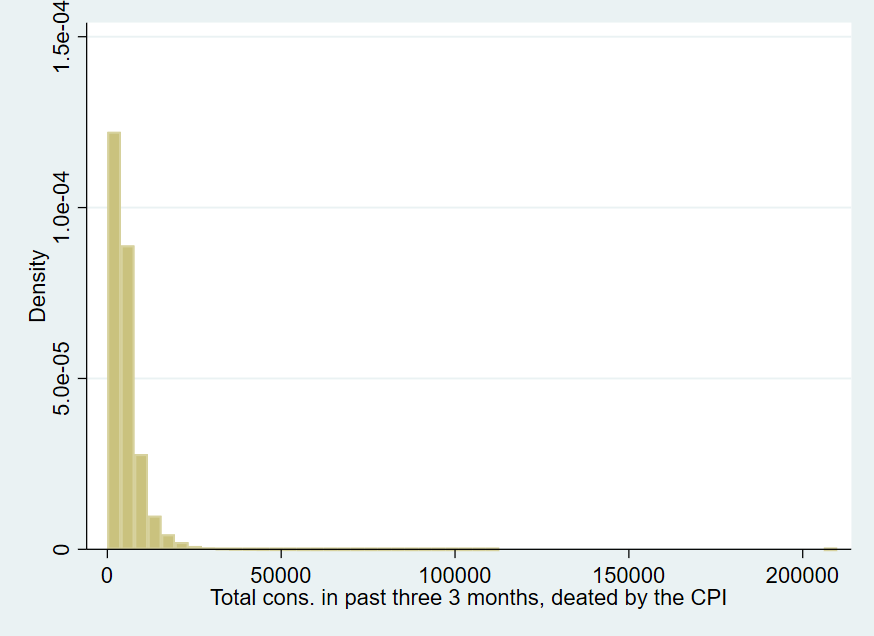
\includegraphics[width=8cm]{graphs/totcons.png}
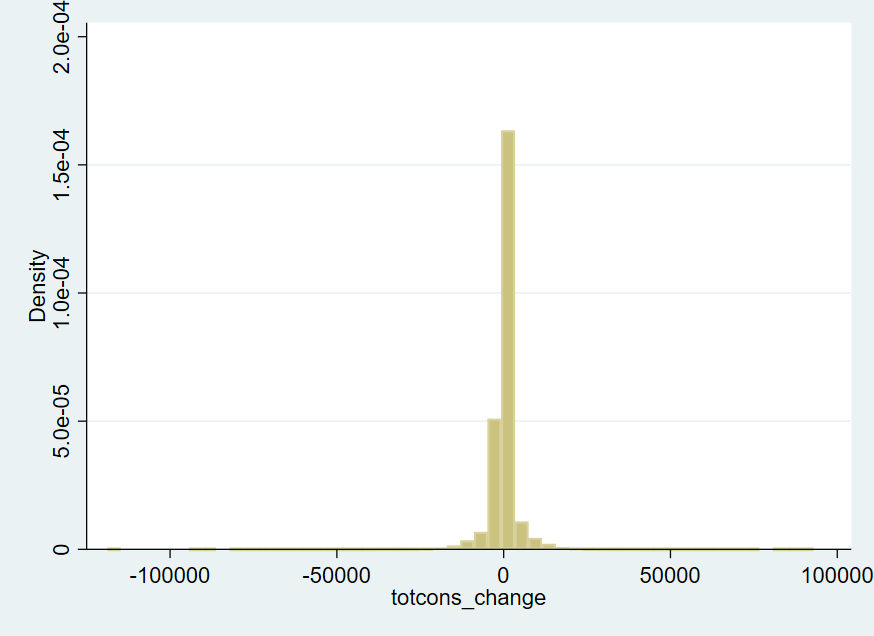
\includegraphics[width=8cm]{graphs/totcons_change.png}\\
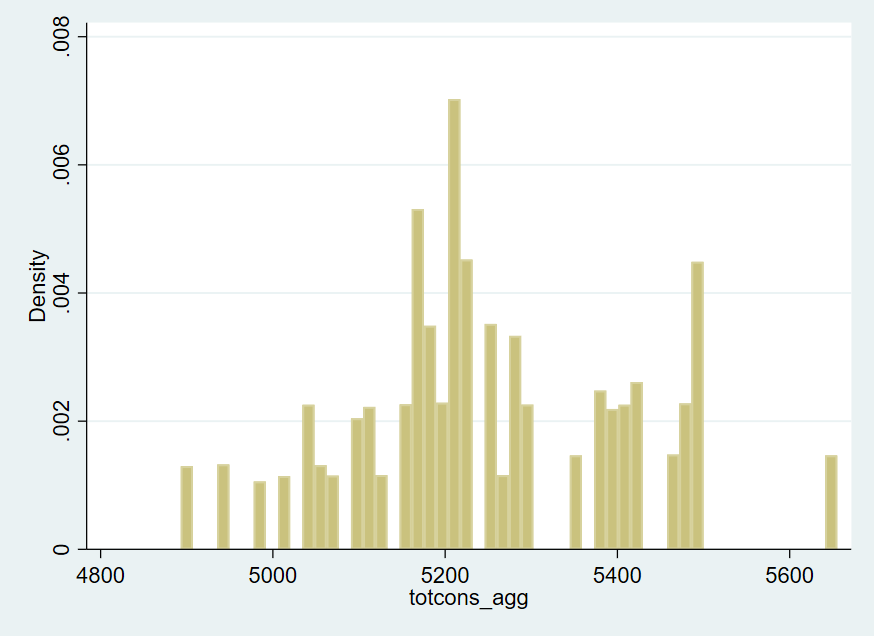
\includegraphics[width=8cm]{graphs/totcons_agg.png}
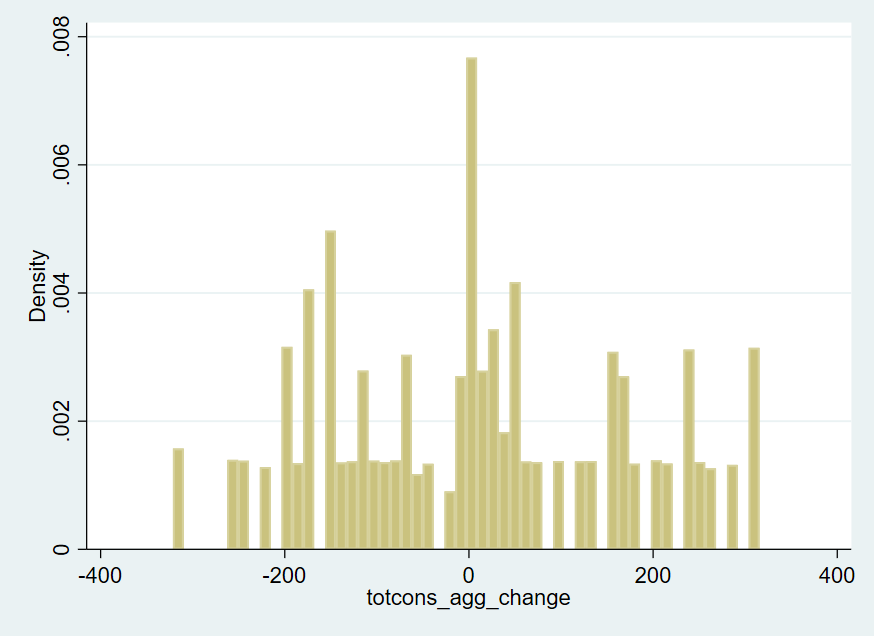
\includegraphics[width=8cm]{graphs/totcons_agg_change.png}\\
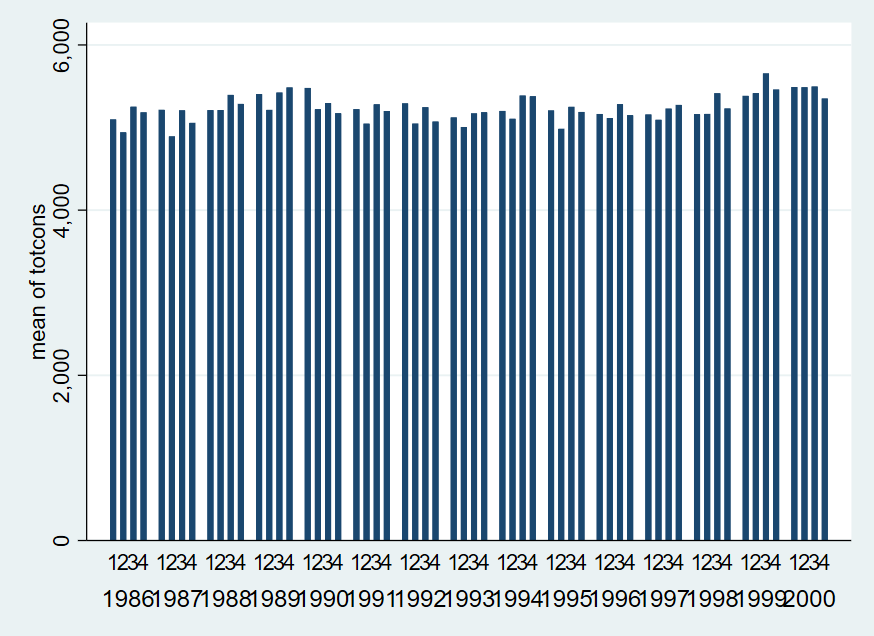
\includegraphics[width=8cm]{graphs/totcons_quarterly.png}
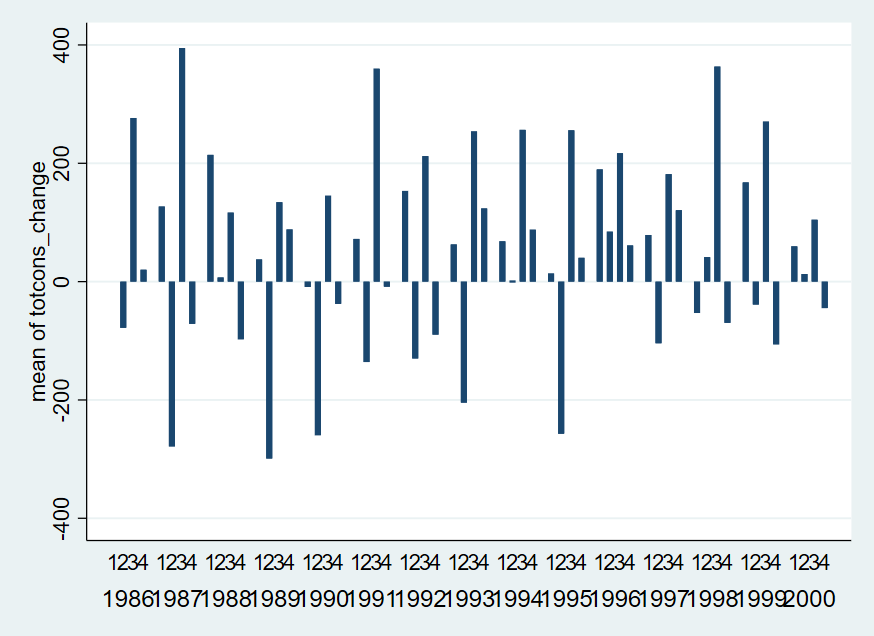
\includegraphics[width=8cm]{graphs/totcons_change_quarterly.png}\\
\end{center}

\subsubsection*{Food}
\begin{center}
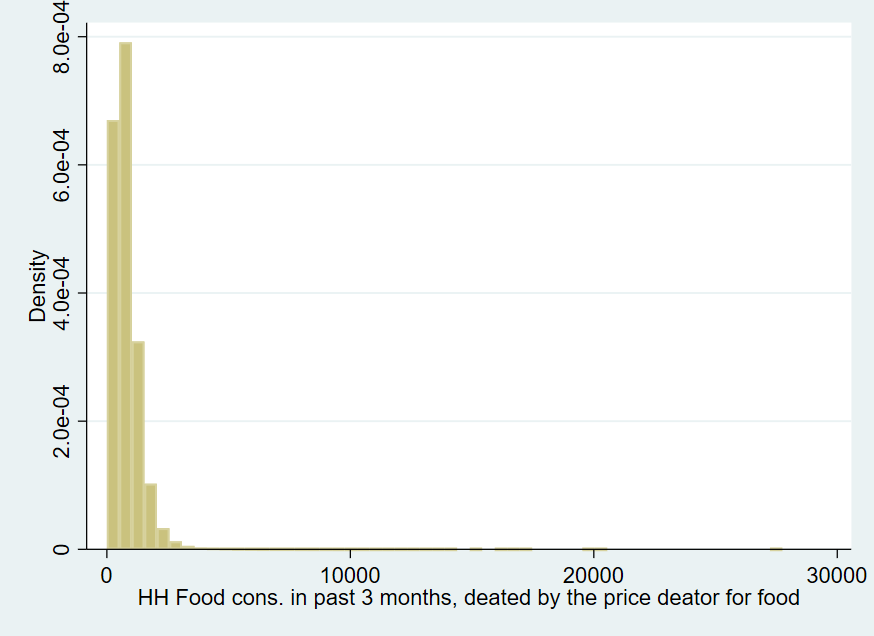
\includegraphics[width=8cm]{graphs/food.png}
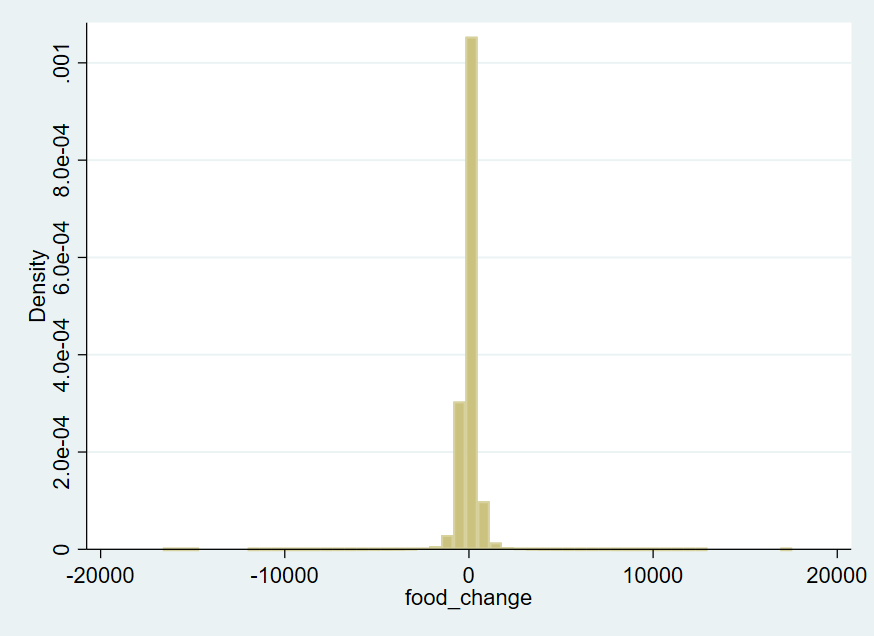
\includegraphics[width=8cm]{graphs/food_change.png}\\
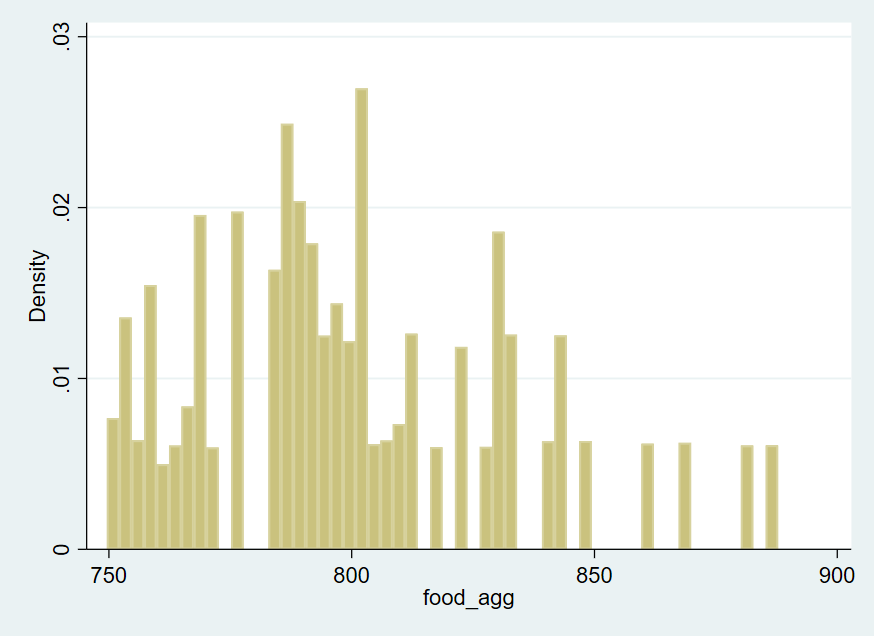
\includegraphics[width=8cm]{graphs/food_agg.png}
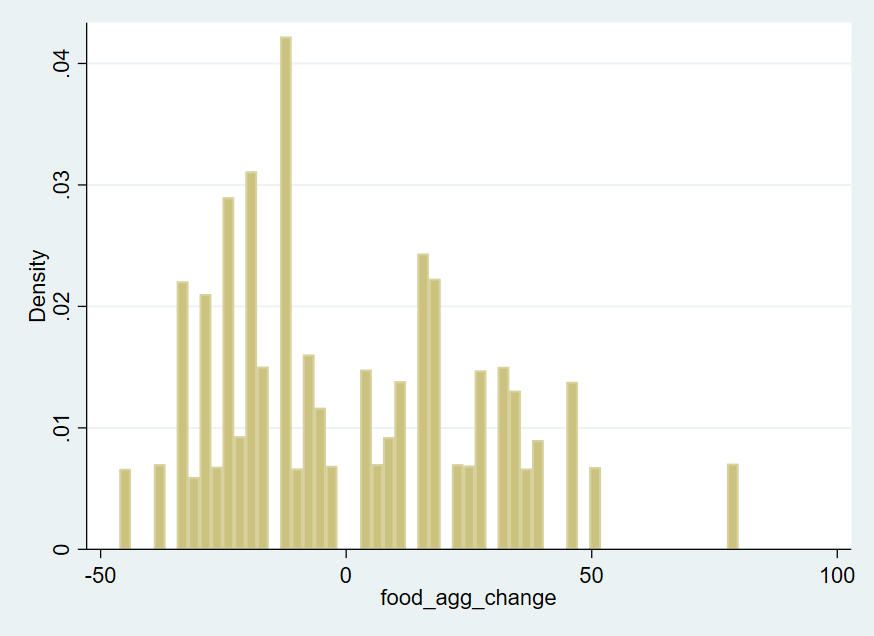
\includegraphics[width=8cm]{graphs/food_agg_change.png}\\
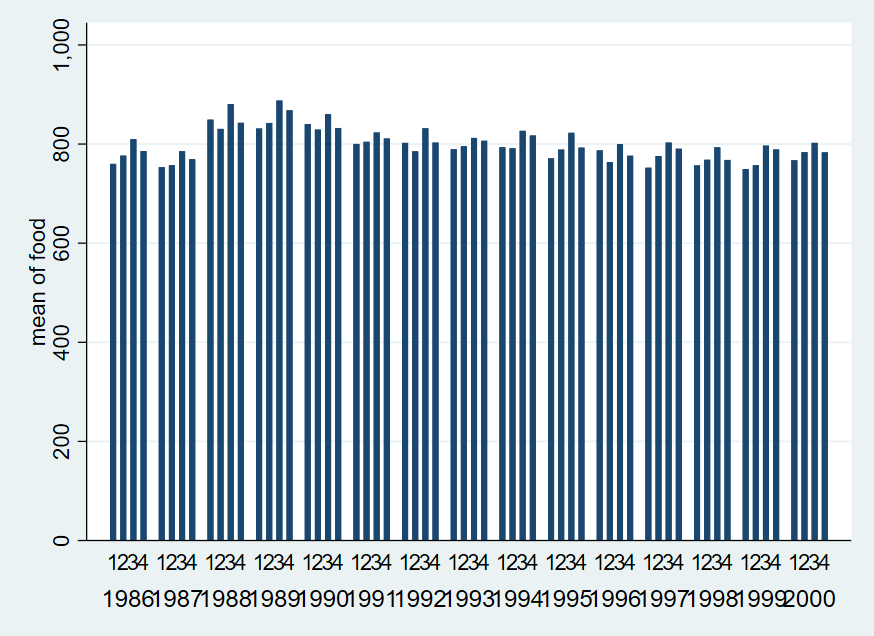
\includegraphics[width=8cm]{graphs/food_quarterly.png}
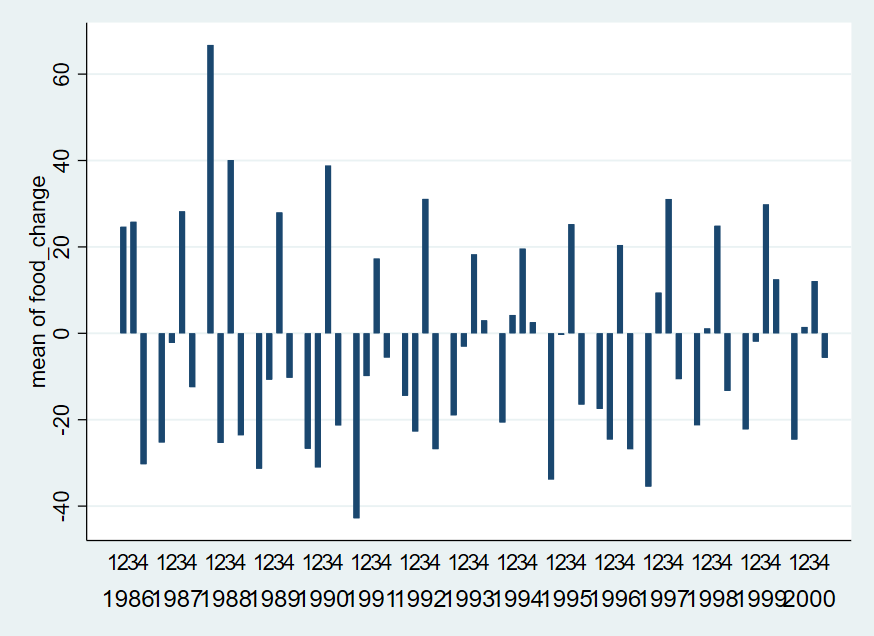
\includegraphics[width=8cm]{graphs/food_change_quarterly.png}\\
\end{center}

\subsubsection*{Nondurable consumption expenditures}
\begin{center}
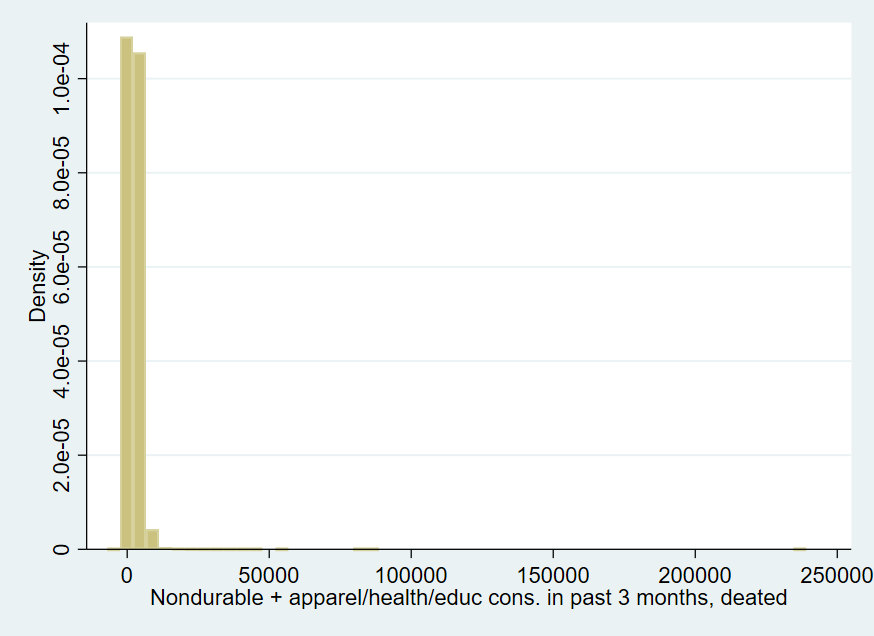
\includegraphics[width=8cm]{graphs/ndcons1.png}
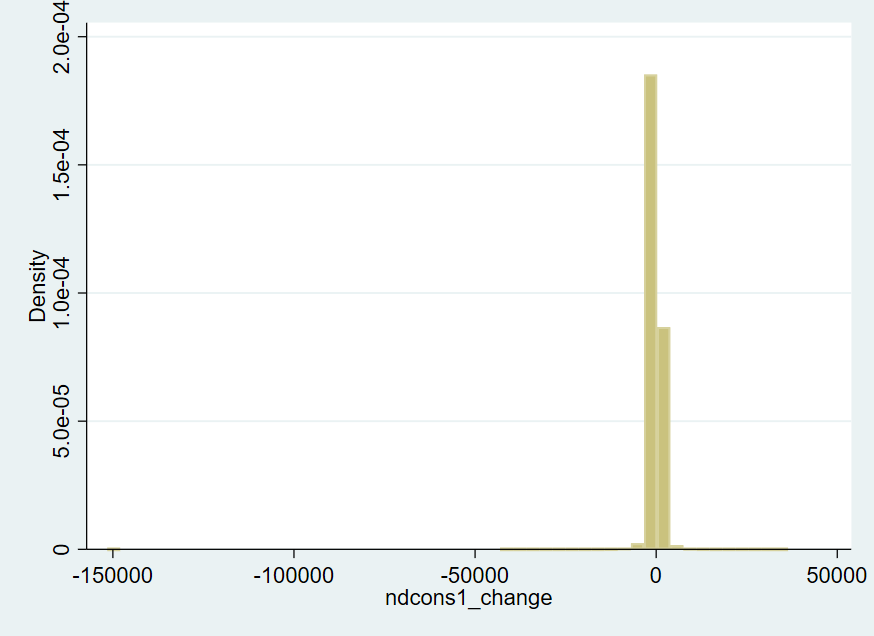
\includegraphics[width=8cm]{graphs/ndcons1_change.png}\\
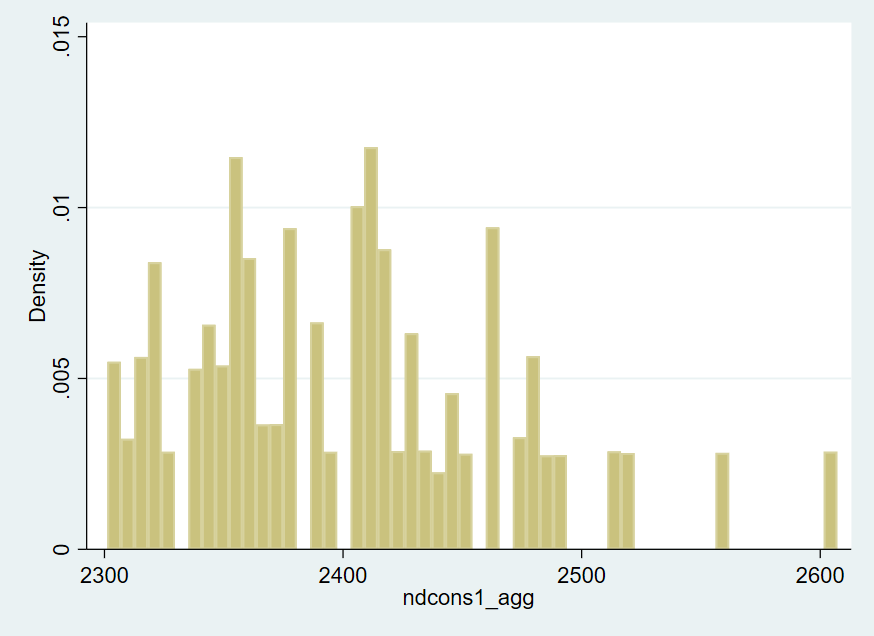
\includegraphics[width=8cm]{graphs/ndcons1_agg.png}
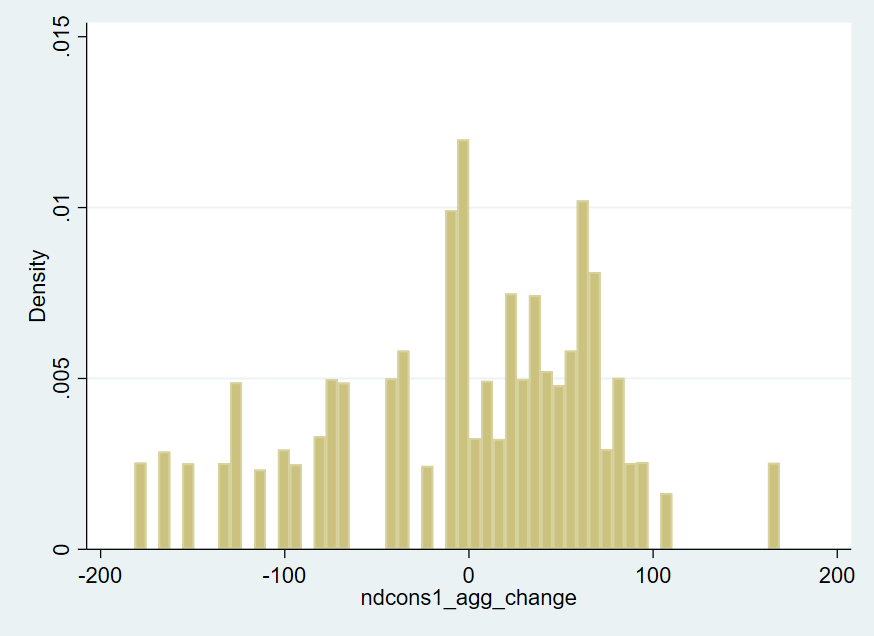
\includegraphics[width=8cm]{graphs/ndcons1_agg_change.png}\\
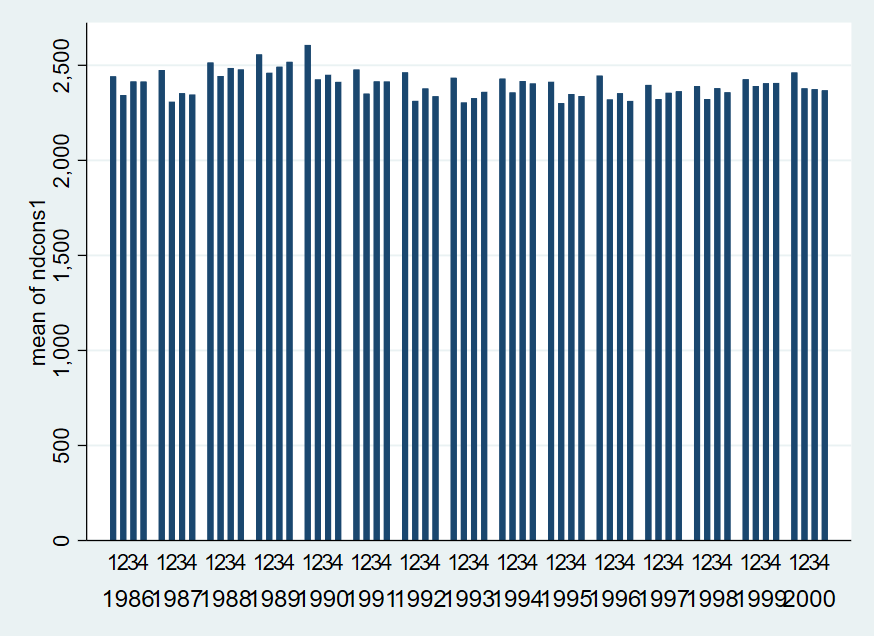
\includegraphics[width=8cm]{graphs/ndcons1_quarterly.png}
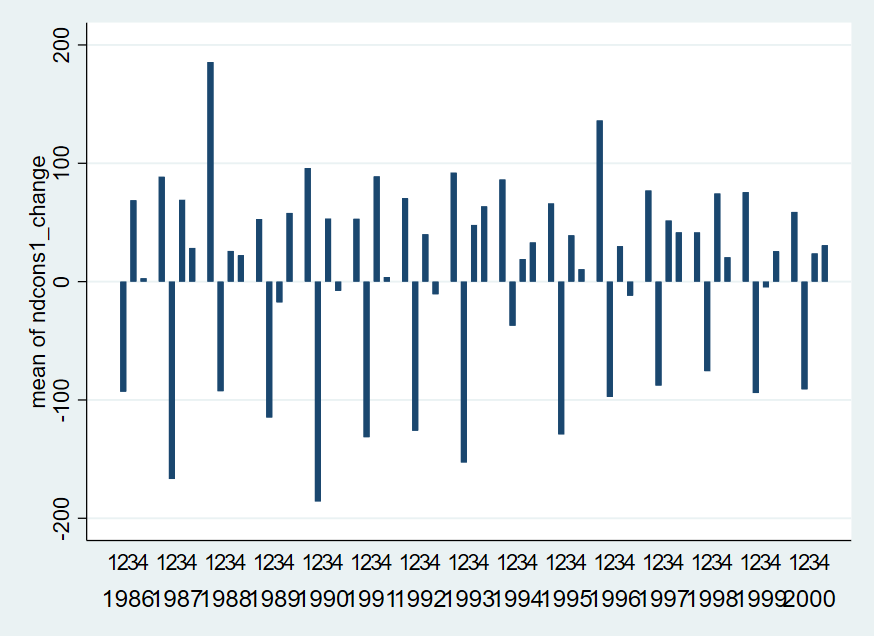
\includegraphics[width=8cm]{graphs/ndcons1_change_quarterly.png}\\
\end{center}


\subsubsection*{Strictly nondurable consumption expenditures}
\begin{center}
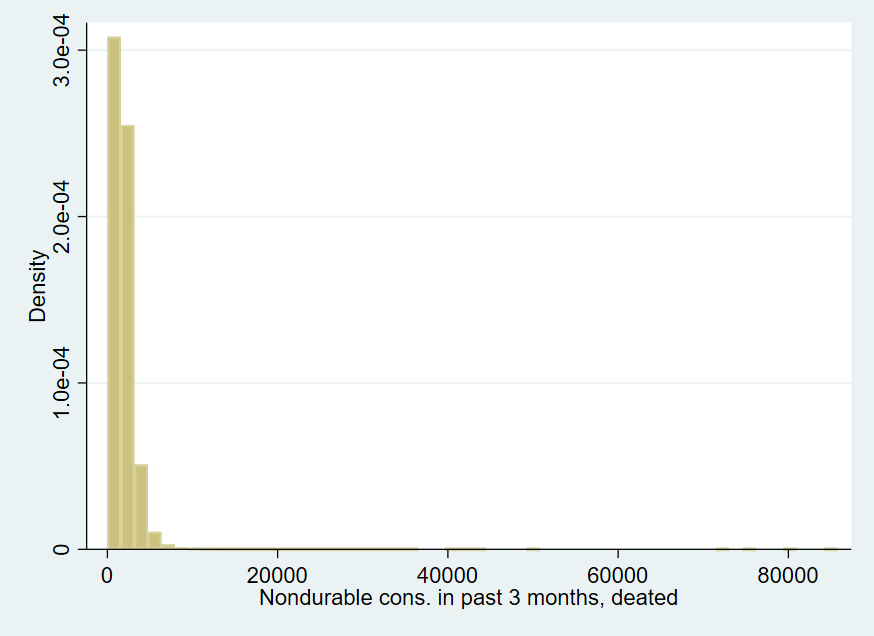
\includegraphics[width=8cm]{graphs/ndcons2.png}
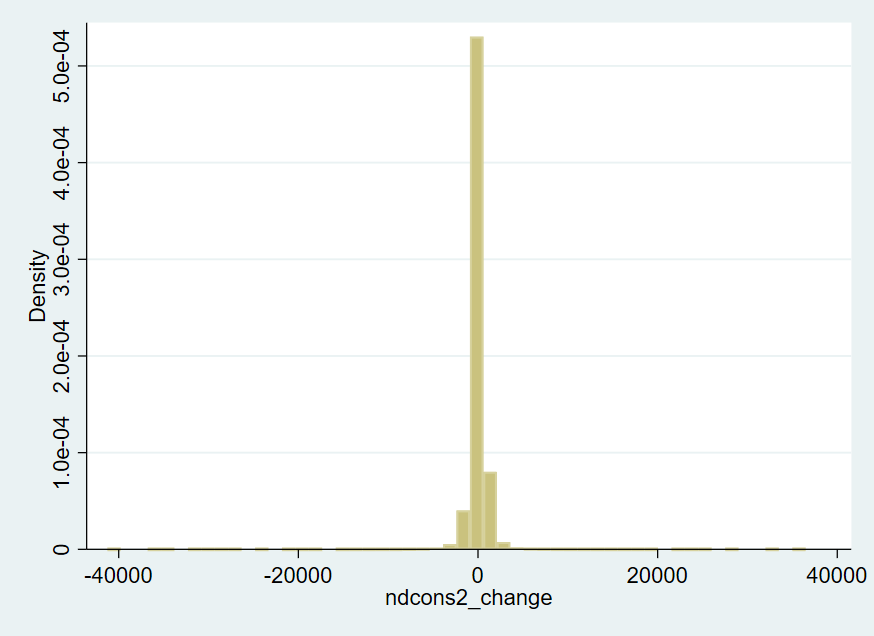
\includegraphics[width=8cm]{graphs/ndcons2_change.png}\\
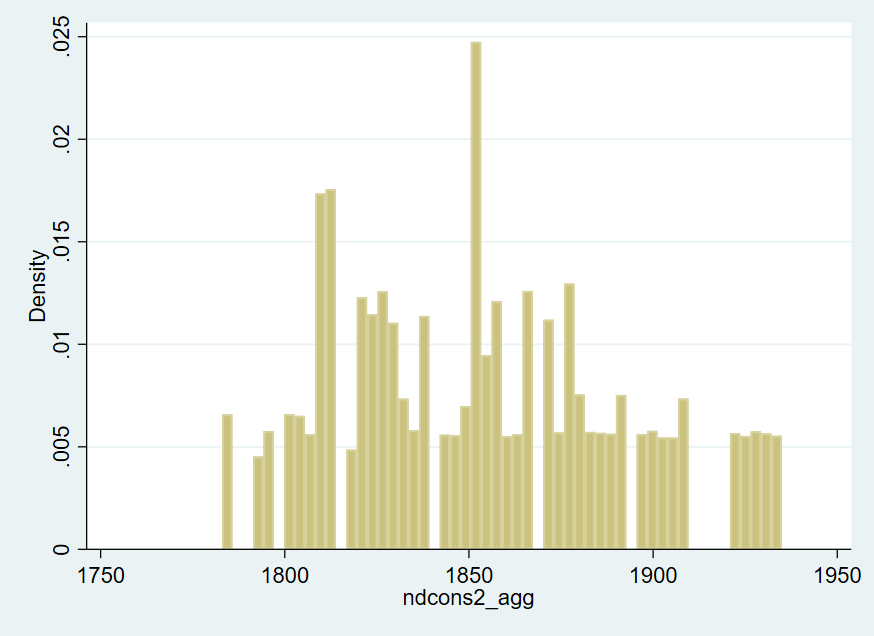
\includegraphics[width=8cm]{graphs/ndcons2_agg.png}
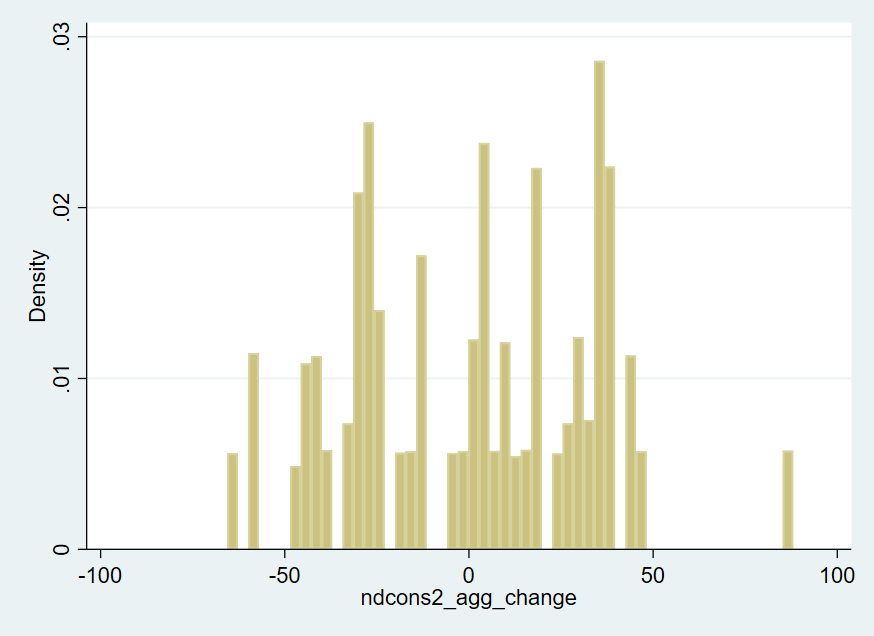
\includegraphics[width=8cm]{graphs/ndcons2_agg_change.png}\\
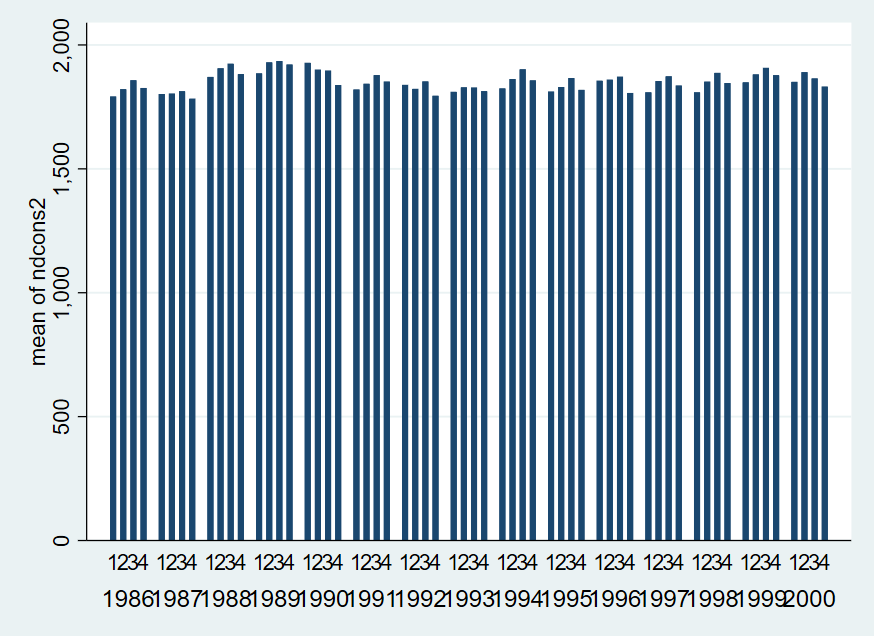
\includegraphics[width=8cm]{graphs/ndcons2_quarterly.png}
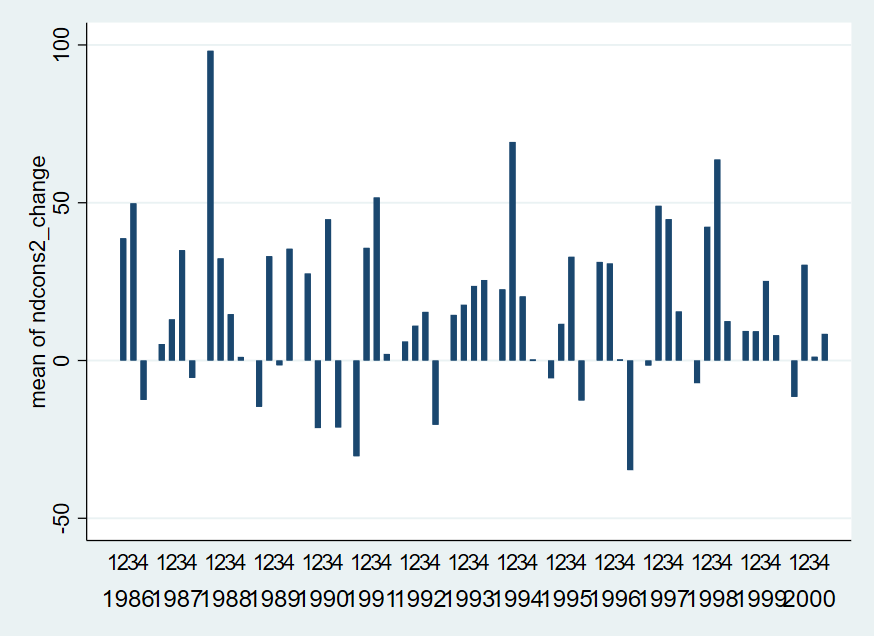
\includegraphics[width=8cm]{graphs/ndcons2_change_quarterly.png}\\
\end{center}

\subsubsection*{Nondurables plus imputed service flows from consumer durables}
\begin{center}
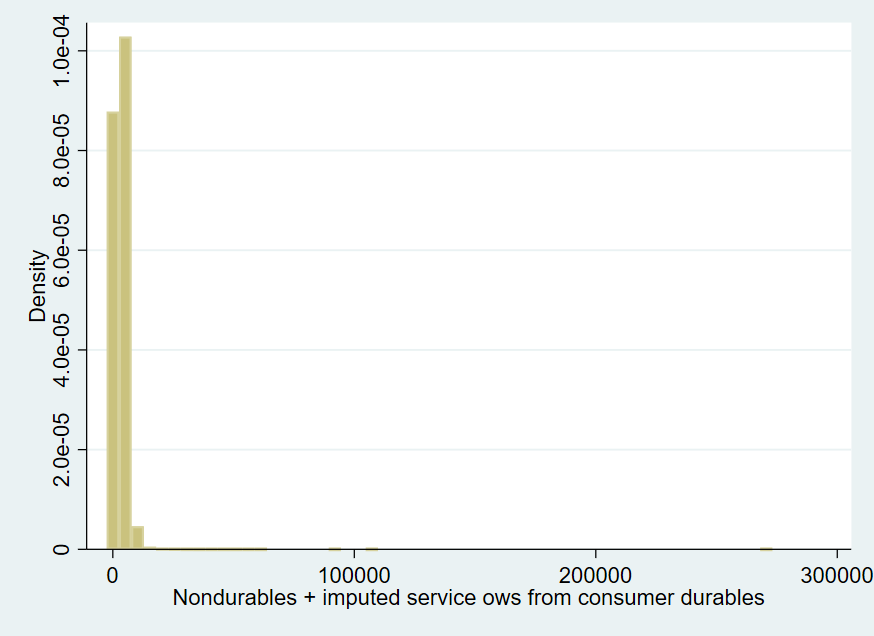
\includegraphics[width=8cm]{graphs/ndconsserv.png}
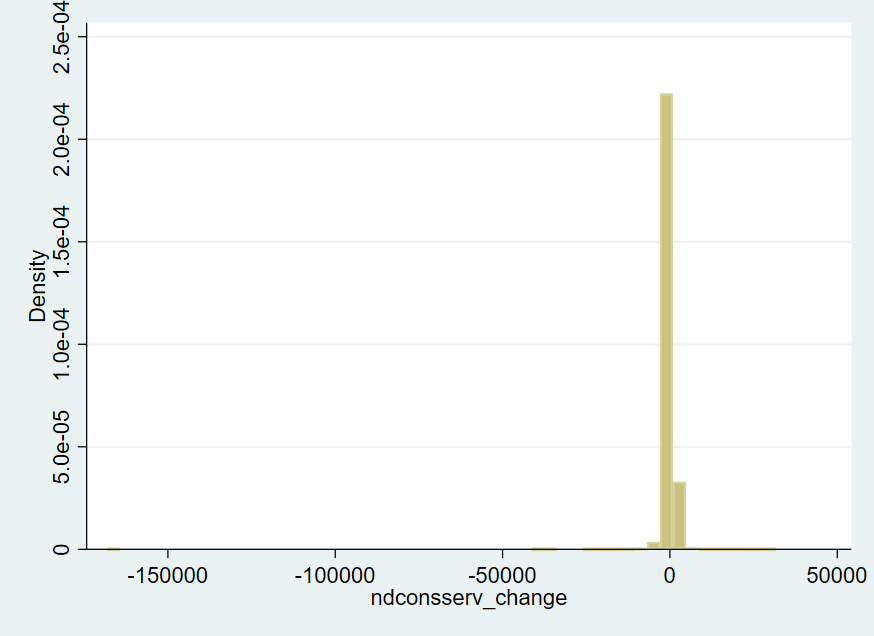
\includegraphics[width=8cm]{graphs/ndconsserv_change.png}\\
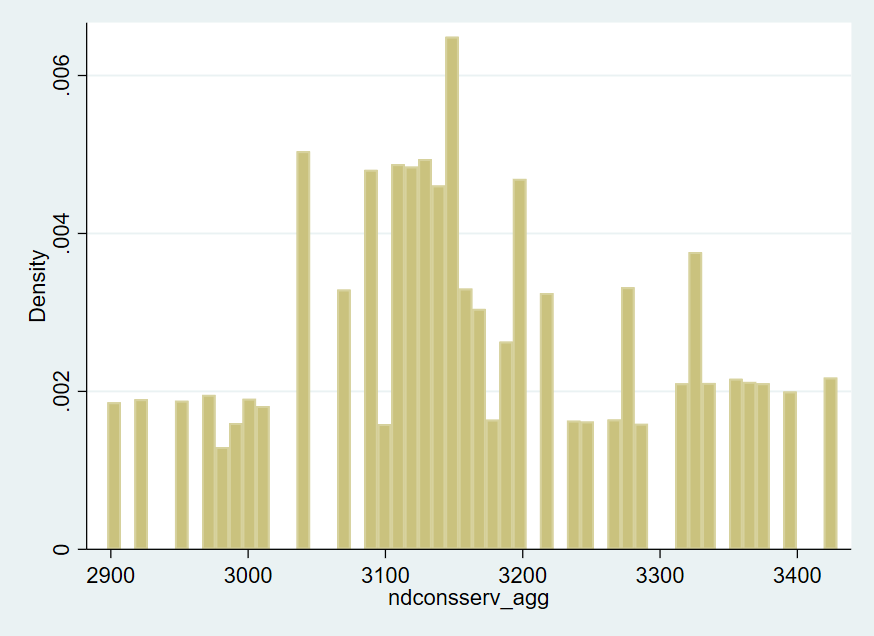
\includegraphics[width=8cm]{graphs/ndconsserv_agg.png}
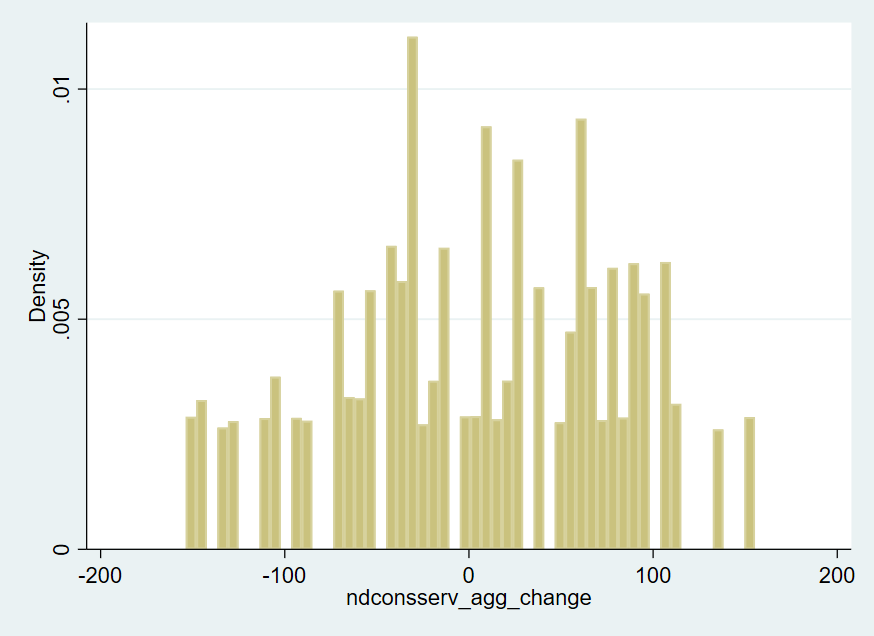
\includegraphics[width=8cm]{graphs/ndconsserv_agg_change.png}\\
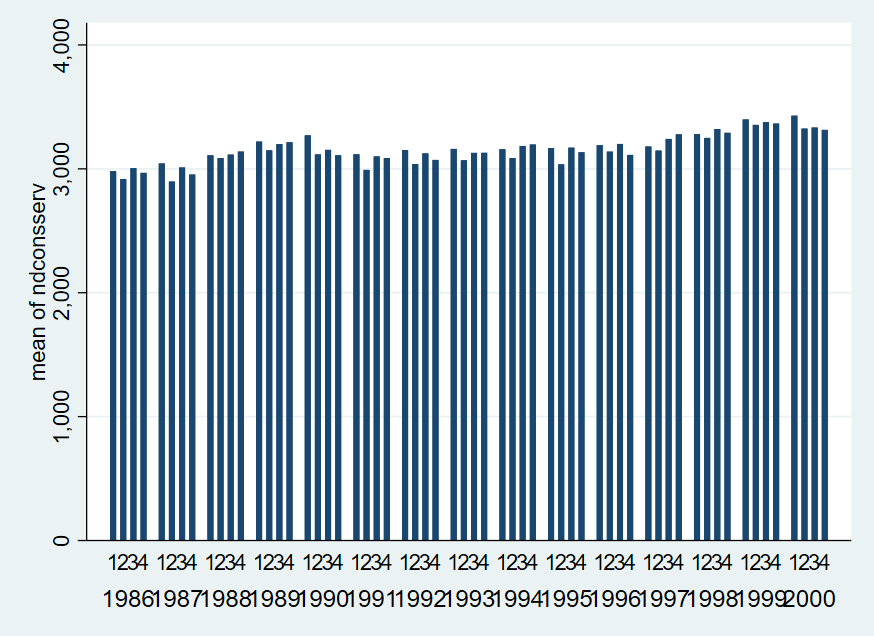
\includegraphics[width=8cm]{graphs/ndconsserv_quarterly.png}
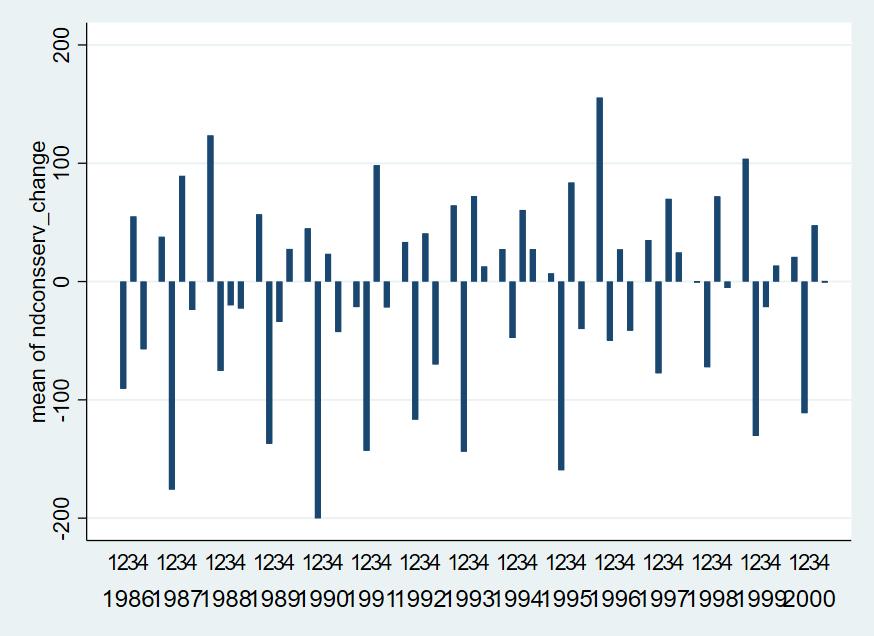
\includegraphics[width=8cm]{graphs/ndconsserv_change_quarterly.png}\\

\end{center}
\subsubsection*{Household income before taxes}
\begin{center}
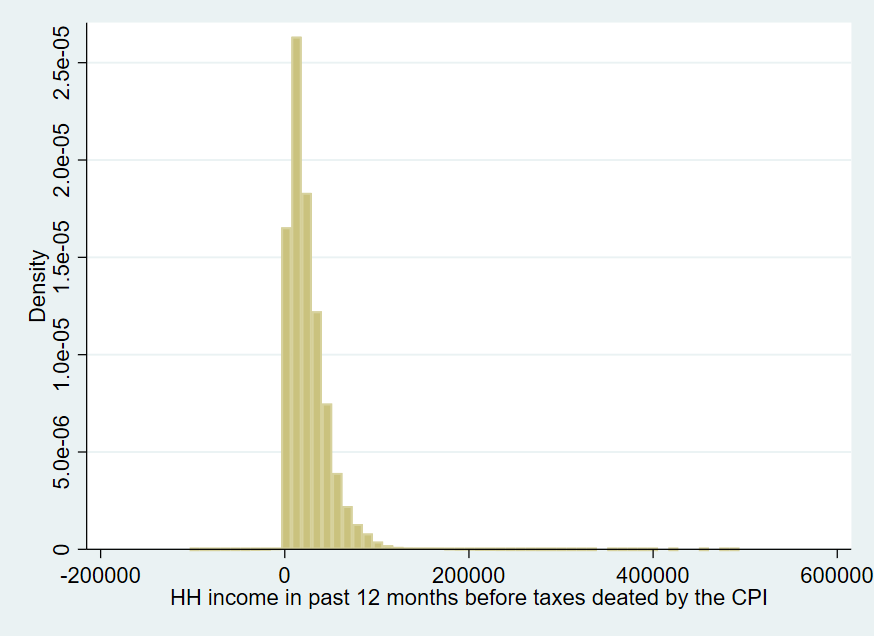
\includegraphics[width=8cm]{graphs/grinc.png}
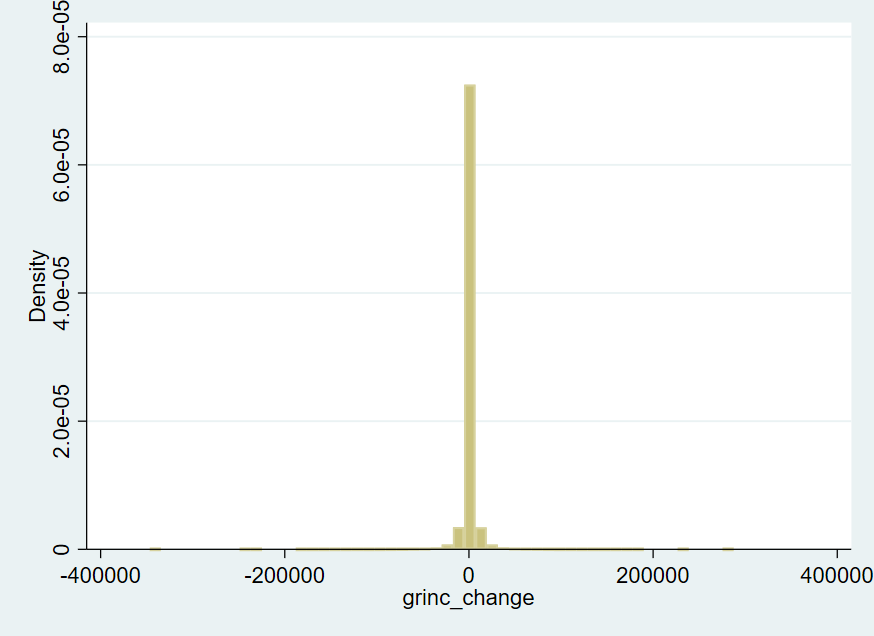
\includegraphics[width=8cm]{graphs/grinc_change.png}\\
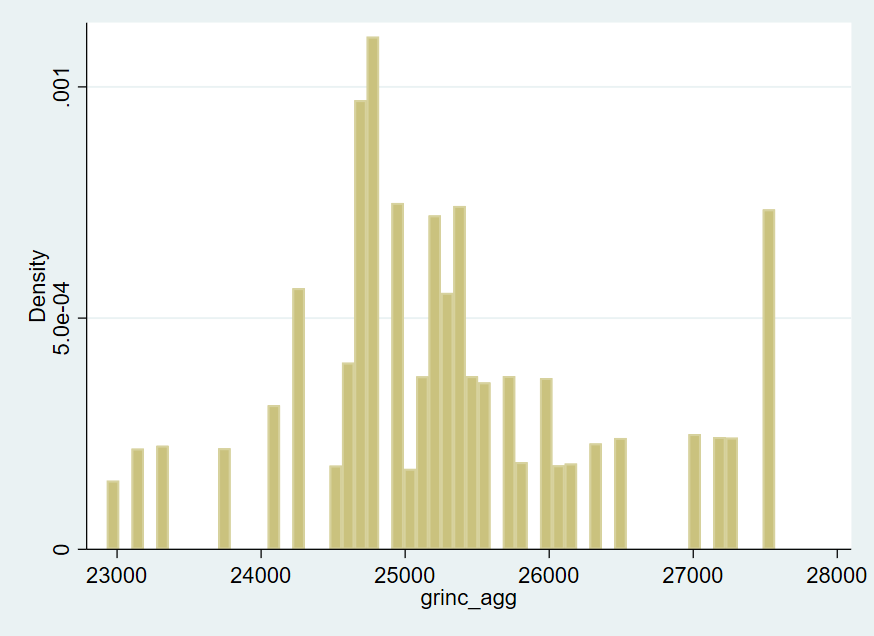
\includegraphics[width=8cm]{graphs/grinc_agg.png}
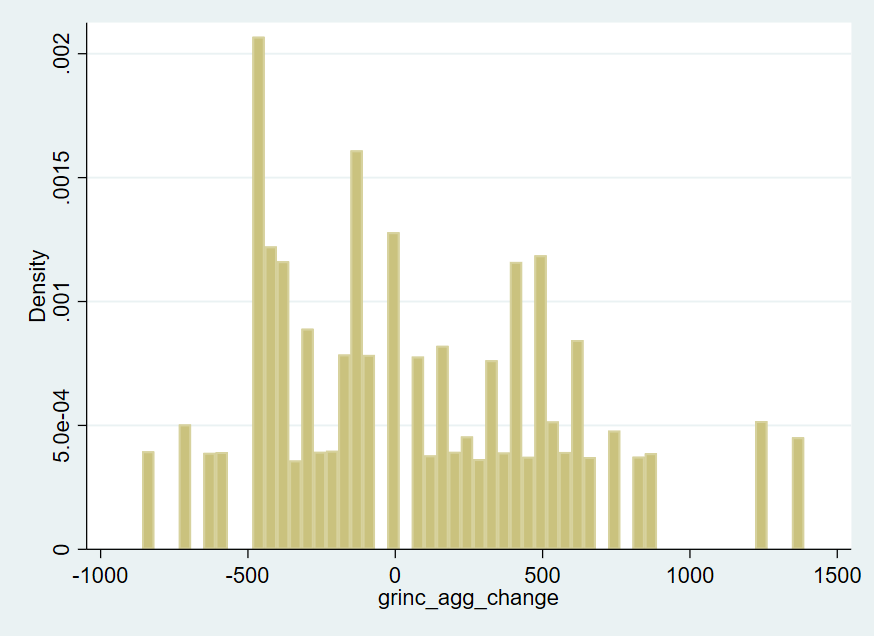
\includegraphics[width=8cm]{graphs/grinc_agg_change.png}\\
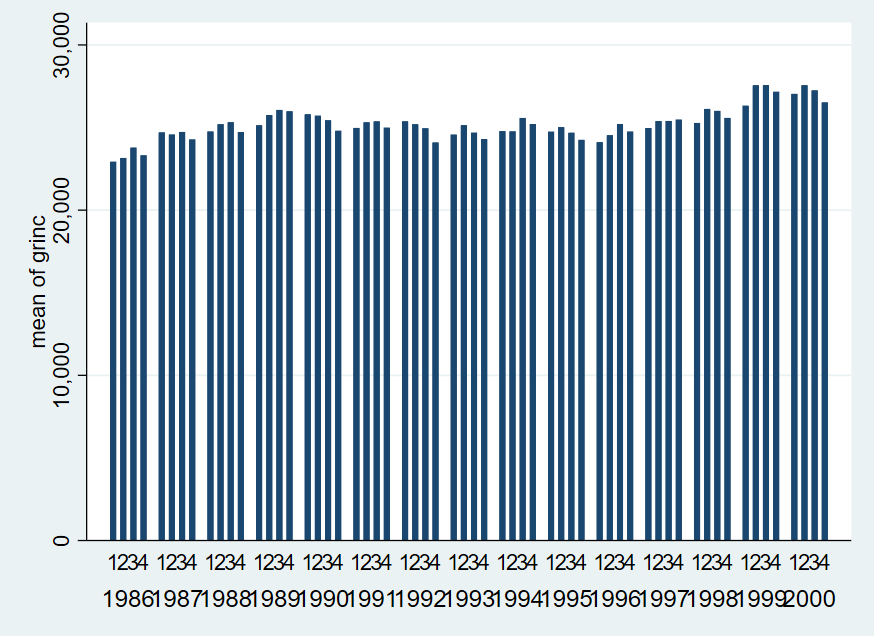
\includegraphics[width=8cm]{graphs/grinc_quarterly.png}
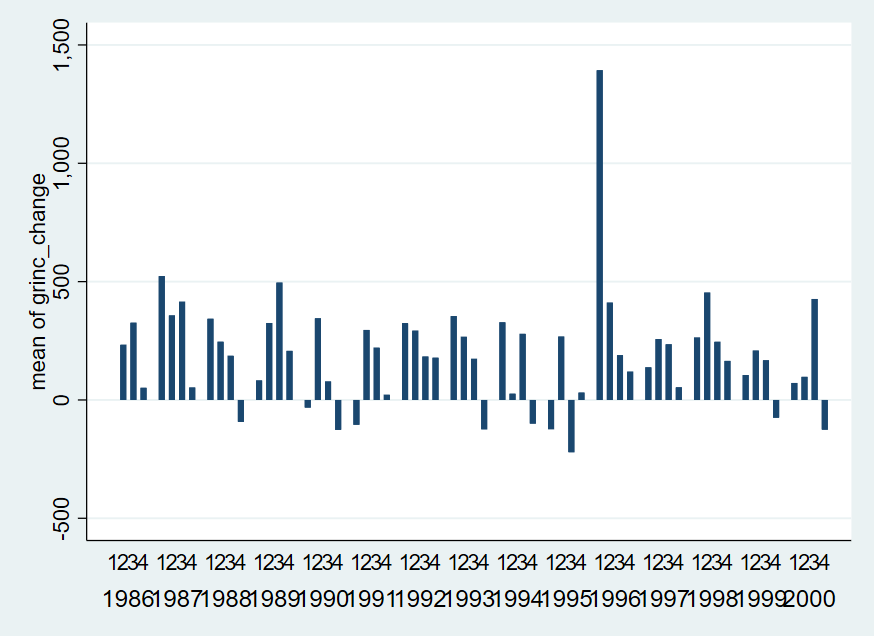
\includegraphics[width=8cm]{graphs/grinc_change_quarterly.png}\\
\end{center}

\subsubsection*{Household income after taxes}
\begin{center}
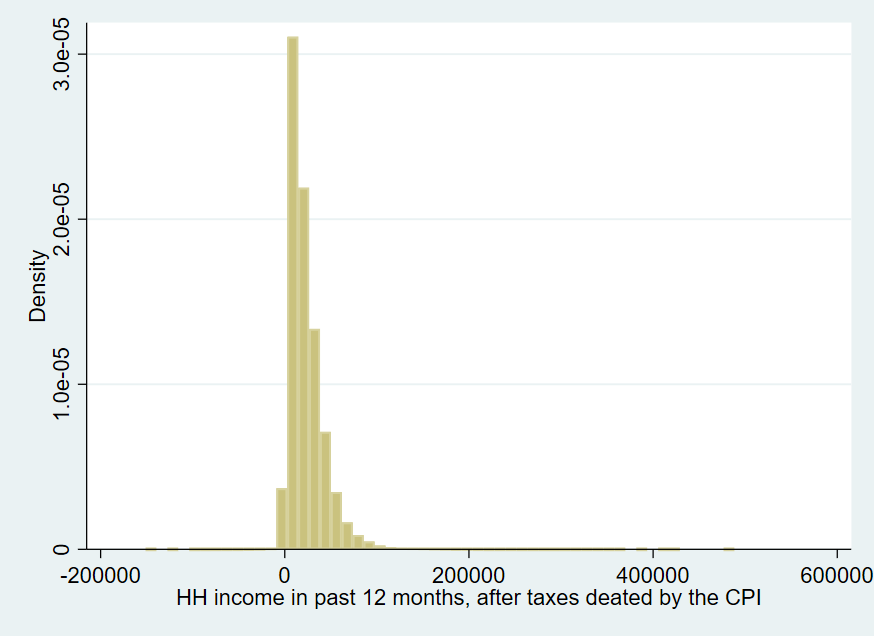
\includegraphics[width=8cm]{graphs/netinc.png}
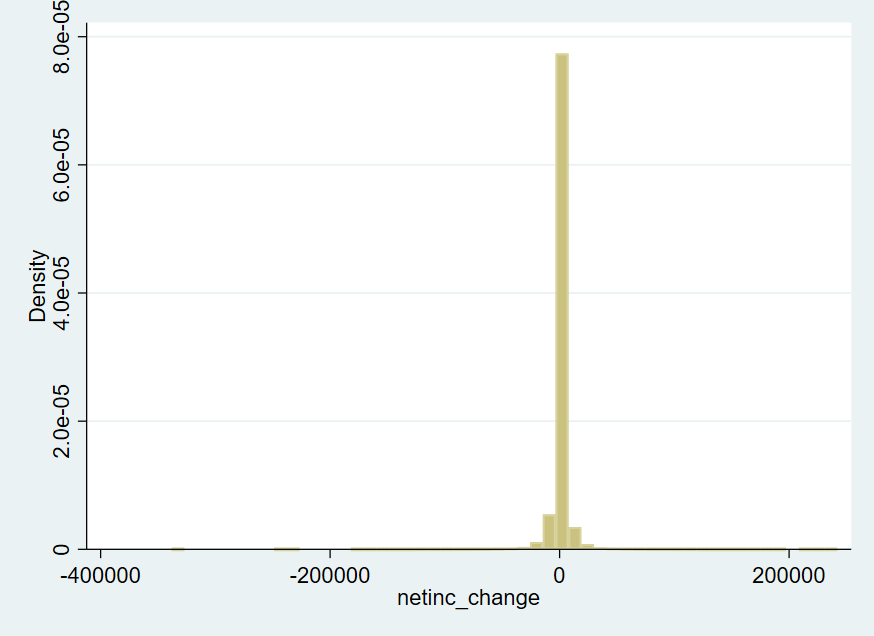
\includegraphics[width=8cm]{graphs/netinc_change.png}\\
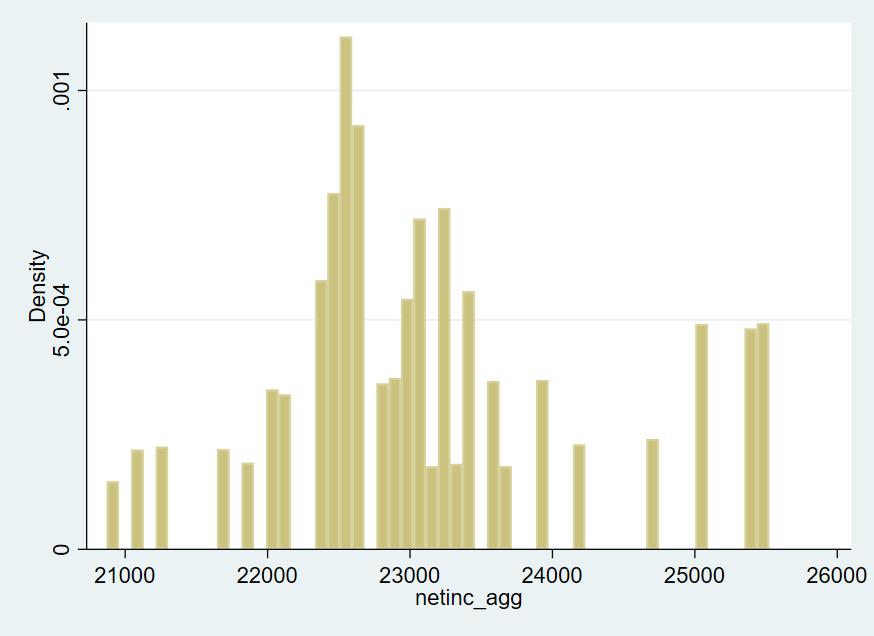
\includegraphics[width=8cm]{graphs/netinc_agg.png}
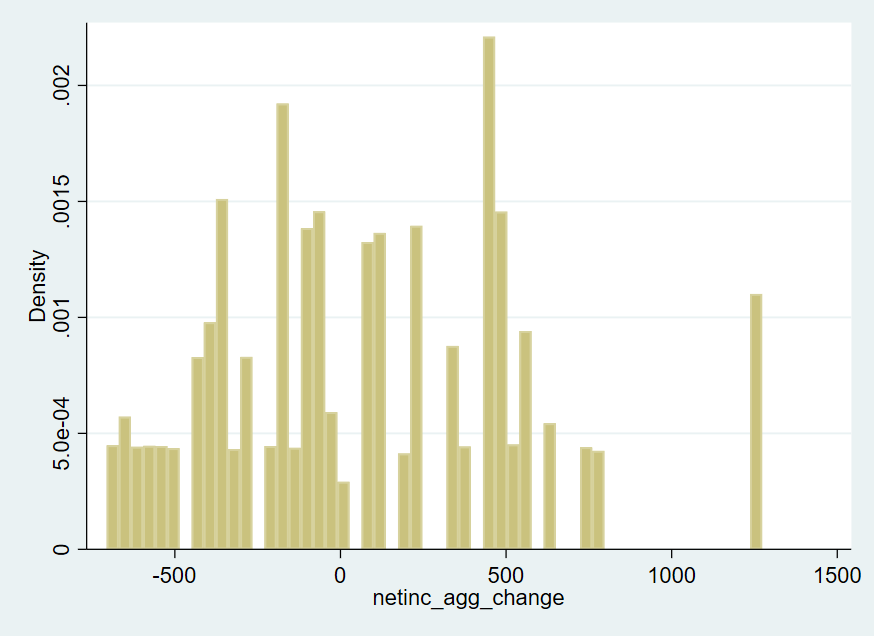
\includegraphics[width=8cm]{graphs/netinc_agg_change.png}\\
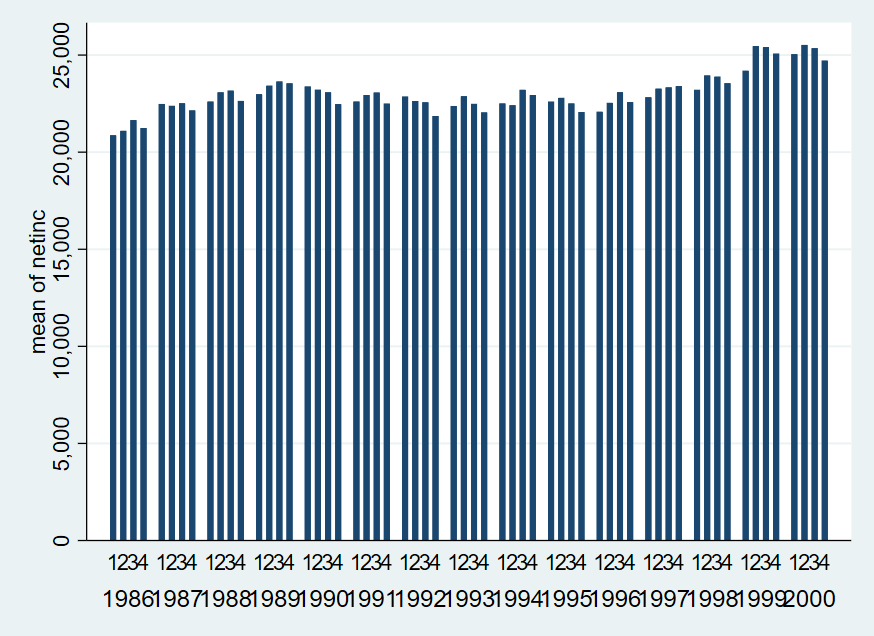
\includegraphics[width=8cm]{graphs/netinc_quarterly.png}
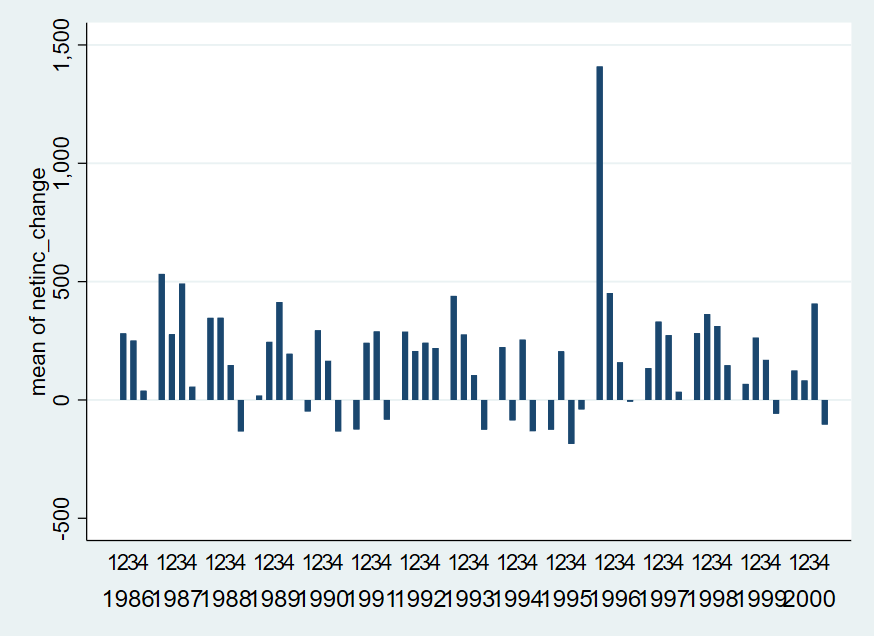
\includegraphics[width=8cm]{graphs/netinc_change_quarterly.png}\\
\end{center}

\subsubsection*{GDP, recessions, income and consumption}
To detect business cycle effects we plotted (i) total income changes in comparison with GDP changes and NBER recessions in the given time span as well as (ii) consumption changes in comparison with GDP changes and NBER recessions in the given time span. We can see fluctuations during recessions, yet, they are not considerably different in magnitute from other occuring fluctuations.

\begin{center}
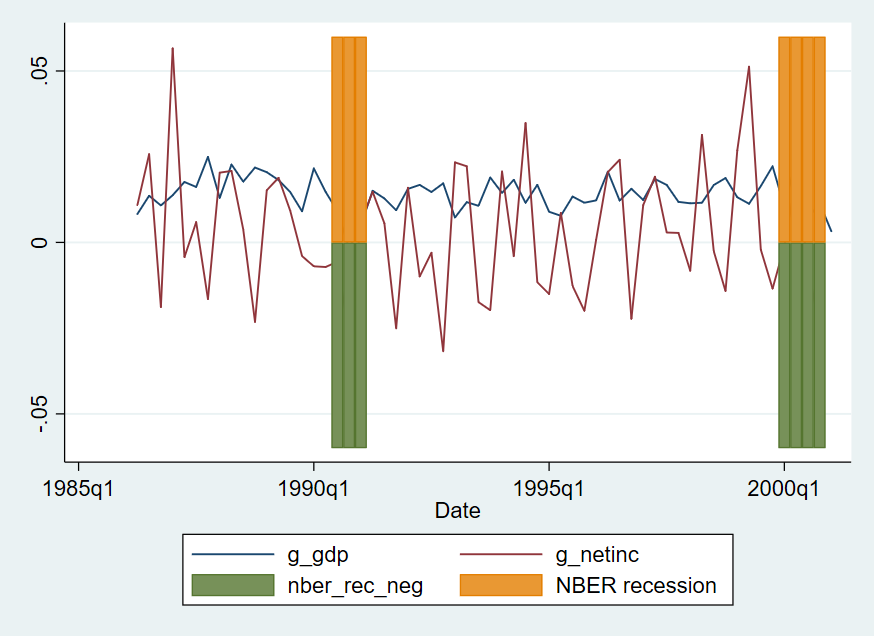
\includegraphics[width=14cm]{graphs/inc_gdp.png}\\
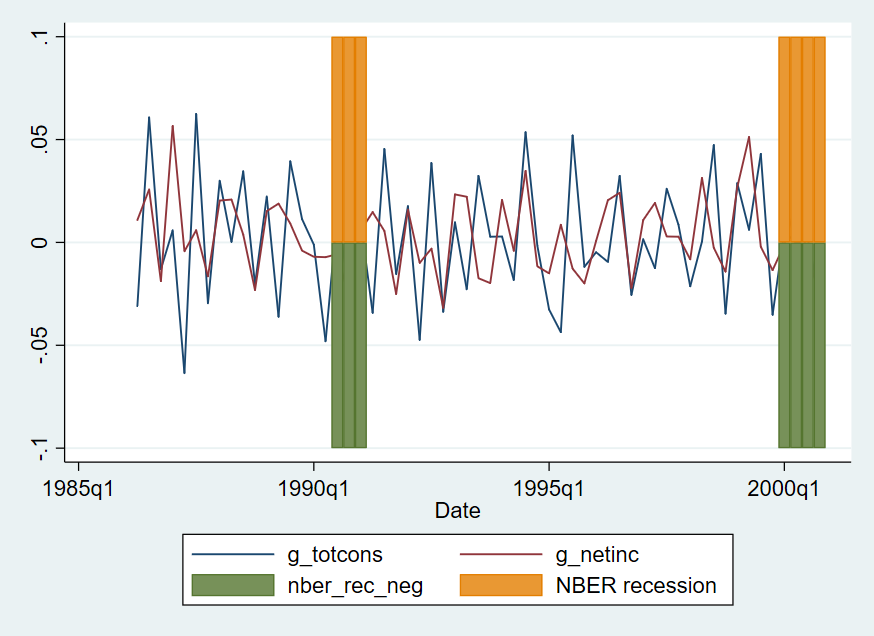
\includegraphics[width=14cm]{graphs/inc_cons.png}\\
\end{center}

%%%%%%%%%%%%%%%%%%%%%%%%%%%%%%%%%%%%%%%%%%%%%%%%%%%%%%%%%%%%%%%%%%%%
%%%%%%%%%%%%%%%%%%%%%%%%%%%%%%%%%%%%%%%%%%%%%%%%%%%%%%%%%%%%%%%%%%%%

\section*{Problem 2: }

\textbf{General explanation on how we deal with the data}:

Since from the Mace paper only the second and the fifth interview contain useful income information and we always work with differences, we will focus on those individuals whose income is observed twice (in second and fifth interview). \\

Interviews take place 9 months apart from one another (we confirmed that for all individuals). However, consumption always refers to consumption in the 3 previous months, while income refers to the income in the last 12 months. In order to handle this frequency imbalance for consumption and income data, we are regressing changes in 3-month-long consumption on changes in annual income (in both cases, the reported changes are calculated with information that is collected 9 months apart). Since 3 month-changes is 1/4 of yearly changes, in order to interpret the magnitude of the effect of income changes, we have to divide the coefficient on income by 4.\\


Our solution to this problem consists of 2 subsections:
\begin{itemize}
    \item In the first subsection, we test for the perfect risk sharing hypothesis, namely, individual consumption depends only on aggregate spending/ consumption. In order to test this hypothesis, we employed the specification from \citealp{mace1991} which is given as follows:
\begin{equation}\label{one}
      \Delta C_t^J =\beta_1 \Delta C_t^a + \beta_2 \Delta y_t^J + u_t^J
\end{equation}
where $\Delta C_t^J$ is the change in individual j's consumption, $\Delta C_t^a$ is the change of aggregate income, $\Delta y_t^J$ is the change in individual j's income. This specification applies to households with exponential utility.

\item In the second subsection, we test whether individual log consumption growth depends only on aggregate log consumption growth. In order to test this hypothesis, we employed the specification from \citealp{mace1991} which is given as follows:

\begin{equation}\label{two}
      \Delta log  C_t^J =\beta_1 \Delta log C_t^a + \beta_2 \Delta log y_t^J + v_t^J
\end{equation}
where   $\Delta log  C_t^J$ is the log growth of individual j's consumption,   $  \Delta log  C_t^a$ is the log growth of aggregate consumption,  $ \Delta log y_t^J$ is the log growth of  individual j's income. This specification applies to households with power utility. \\

$\Delta log  C_t^a$ are computed as in \citealp{mace1991}:

\begin{equation}\label{two}
      \Delta log  C_t^a = \frac{1}{J} \sum_{J}^{J=1} \Delta log  C_t^J
\end{equation}.

That is, the average across households of log-differences of consumption. \\

Following this, we will re-estimate her results (as well as we possibly can, as we don’t observe employment status) using CEX dataset for both specifications. In both cases, we introduce some additional controls to extend the model and review alternative economic interpretations. We present the regression tables and comment on the F-tests testing the joint hypothesis on the coefficients on aggregate consumption changes (growth) and individual income changes (growth).
\end{itemize}


%%%%%%%%%%%%%%%%%%%%%%%%%%%%%%%%%%%%%%%%%%%%%%%%%%%%%%%%%%%%%%%%%%%%
\section*{Hypothesis 1: Individual Consumption depends only on Aggregate Spending}
From equation \eqref{one}, the predictions of risk sharing model are $\beta_1=1$ \& $\beta_2=0$, we would expect the coefficient on diff\_netinc to be 0 and coefficients on different types of consumption(avg-food-change, avg-ndcons1-change,  avg-ndcons2-change,avg-ndconsserv-change) to be 1. \\

Please note: In all coming specification we will always look at the same type of consumption (i.e. food, non-durables including education, non-durables excluding education, etc.) on the individual and aggregate levels (the exact definitions of the consumption variables are given in  Problem 1). 

\subsection*{Mace's specification}

\begin{table}[!h]\centering
\def\sym#1{\ifmmode^{#1}\else\(^{#1}\)\fi}
\caption{\label{tab:2.1A-deltacons} Explaining changes in consumption}
\begin{tabular}{l*{5}{c}}
\hline\hline
            &\multicolumn{1}{c}{(1)}         &\multicolumn{1}{c}{(2)}         &\multicolumn{1}{c}{(3)}         &\multicolumn{1}{c}{(4)}         &\multicolumn{1}{c}{(5)}         \\
\hline
diff\_netinc &      0.0215\sym{***}&     0.00116\sym{***}&     0.00463\sym{***}&     0.00345\sym{***}&     0.00474\sym{***}\\
            &   (0.00137)         &  (0.000195)         &  (0.000498)         &  (0.000339)         &  (0.000526)         \\
avg-totcons-change&       1.000\sym{***}&                     &                     &                     &                     \\
            &    (0.0628)         &                     &                     &                     &                     \\
avg-food-change&                     &       1.005\sym{***}&                     &                     &                     \\
            &                     &    (0.0570)         &                     &                     &                     \\
avg-ndcons1-change&                     &                     &       0.998\sym{***}&                     &                     \\
            &                     &                     &    (0.0534)         &                     &                     \\
avg-ndcons2-change&                     &                     &                     &       1.000\sym{***}&                     \\
            &                     &                     &                     &    (0.0639)         &                     \\
avg-ndconsserv-change&                     &                     &                     &                     &       0.999\sym{***}\\
            &                     &                     &                     &                     &    (0.0568)         \\
constant    &      -12.35         &      -0.645         &      -2.549         &      -1.969         &      -2.701         \\
            &     (24.92)         &     (2.764)         &     (7.347)         &     (6.008)         &     (7.435)         \\
\hline
\(N\)       &       44772         &       44772         &       44772         &       44772         &       44772         \\
\hline\hline
\multicolumn{6}{l}{\footnotesize Standard errors in parentheses}\\
\multicolumn{6}{l}{\footnotesize \sym{*} \(p<0.05\), \sym{**} \(p<0.01\), \sym{***} \(p<0.001\)}\\
\end{tabular}
\end{table}


In table \ref{tab:2.1A-deltacons}, we can see that the coefficient of diff\_netinc is close to 0, on the other hand, coefficients on the 4 different types of consumption change as well as on total consumption change are close to 1. All of these coefficients are statistically significant at $1\%$ level. Across the variables that our dataset has in common with Mace's (total consumption, non-durables, food), we find the coefficients on those variables from our regression and hers are roughly the same. 

In contrast, using F test, Mace found the coefficients significant when she regressed individual's Non-durables consumption change on average Non-durables consumption change. Our specification of the F-tests all indicate p-values of under 0.001, \textcolor{red}{rejecting} that (using this exponential utility specification), the results are in line with what is predicted by the risk sharing hypothesis This difference may be due to the fact that she tested the hypothesis using a different dataset and including the control for changes in employment status. In the next section we introduce additional controls to verify if not some other explanatory variable was driving the observed results.

\subsection*{Our additional controls}

In table \ref{tab:2.1B-deltacons-net} , some additional variables are introduced into the model: dummy variables for 4 quarters, age and household size (hhzsize). The reason why we include dummy variables for 4 quarters is to control for the seasonality of consumption, i.e. aggregate consumption as well as individual level's consumption vary significantly across quarters. We have seem this takes place in the data in Problem 1. Adding quarterly dummy variables should eliminate any omitted variable bias that may occur in the previous model. Secondly, age is particularly relevant because, theoretically speaking, older household should have more chances to self-insure by accumulating wealth, since we don't have any wealth data in our dataset, age is a good proxy. (One could also think of adding squared age). Last but not least, different demographic groups have different consumption elasticity as well as different access to insurance. A larger household size means there is a higher likelihood of people of 2 or more demographic groups living in the same house, for example, a couple with two children are far less likely to reduce consumption due to income shock than household of couples with no children or singles.

The F-tests indicate p-values well below the 1\% level, which we again interpret as a clear rejection of Mace's hypothesis. 

\begin{table}[htbp]\centering
\def\sym#1{\ifmmode^{#1}\else\(^{#1}\)\fi}
\caption{\label{tab:2.1B-deltacons-net} Explaining change in consumption - net}
\begin{tabular}{l*{5}{c}}
\hline\hline
            &\multicolumn{1}{c}{(1)}         &\multicolumn{1}{c}{(2)}         &\multicolumn{1}{c}{(3)}         &\multicolumn{1}{c}{(4)}         &\multicolumn{1}{c}{(5)}         \\
\hline
netinc-change&      0.0214\sym{***}&     0.00116\sym{***}&     0.00456\sym{***}&     0.00339\sym{***}&     0.00482\sym{***}\\
            &   (0.00137)         &  (0.000195)         &  (0.000499)         &  (0.000339)         &  (0.000526)         \\
age         &       3.029\sym{*}  &       0.186         &      -0.591         &      -0.682\sym{*}  &       0.360         \\
            &     (1.194)         &     (0.170)         &     (0.434)         &     (0.295)         &     (0.458)         \\
hhsize      &       48.43\sym{***}&       1.231         &       16.36\sym{***}&       15.00\sym{***}&      -20.32\sym{***}\\
            &     (13.33)         &     (1.899)         &     (4.852)         &     (3.299)         &     (5.117)         \\
1.quarter   &           0         &           0         &           0         &           0         &           0         \\
            &         (.)         &         (.)         &         (.)         &         (.)         &         (.)         \\
2.quarter   &      -8.535         &      -0.368         &      -1.240         &      -0.823         &      -3.310         \\
            &     (59.52)         &     (8.210)         &     (22.56)         &     (13.66)         &     (23.67)         \\
3.quarter   &      -7.273         &      -0.407         &      -1.313         &      -0.912         &      -2.234         \\
            &     (56.02)         &     (7.953)         &     (22.09)         &     (13.81)         &     (22.24)         \\
4.quarter   &       12.75         &       0.646         &       3.128         &       2.434         &       1.534         \\
            &     (55.25)         &     (7.834)         &     (23.26)         &     (13.47)         &     (23.45)         \\
year        &    -0.00331         &     0.00111         &     -0.0132         &     -0.0129         &      0.0109         \\
            &     (0.729)         &     (0.105)         &     (0.266)         &     (0.180)         &     (0.280)         \\
avg-totcons-change&       0.996\sym{***}&                     &                     &                     &                     \\
            &    (0.0679)         &                     &                     &                     &                     \\
avg-food-change&                     &       1.002\sym{***}&                     &                     &                     \\
            &                     &    (0.0644)         &                     &                     &                     \\
avg-ndcons1-change&                     &                     &       1.000\sym{***}&                     &                     \\
            &                     &                     &    (0.0641)         &                     &                     \\
avg-ndcons2-change&                     &                     &                     &       0.999\sym{***}&                     \\
            &                     &                     &                     &    (0.0644)         &                     \\
avg-logndconsserv-change&                     &                     &                     &                     &       0.996\sym{***}\\
            &                     &                     &                     &                     &    (0.0659)         \\
constant    &      -290.9\sym{**} &      -13.35         &      -15.28         &      -6.402         &       32.94         \\
            &     (111.0)         &     (15.41)         &     (40.26)         &     (26.85)         &     (41.74)         \\
\hline
\(N\)       &       44772         &       44772         &       44772         &       44772         &       44772         \\
\hline\hline
\multicolumn{6}{l}{\footnotesize Standard errors in parentheses}\\
\multicolumn{6}{l}{\footnotesize \sym{*} \(p<0.05\), \sym{**} \(p<0.01\), \sym{***} \(p<0.001\)}\\
\end{tabular}
\end{table}
. \\

From table \ref{tab:2.1B-deltacons-net}, we can see that the coefficients of interest are still roughly the same and significant. By adding additional controls to the model, which serves as robustness check, the coefficients don't change much in either significance or size. 

Also in this specification The F-tests on indv. income changes and aggregate consumption changes indicate p-values well below the 1\% level, which we interpret as a clear rejection of Mace's hypothesis. 

\subsection*{Our additional controls plus controlling for gross income changes instead of net income changes}
Since net income changes may be correlated with household size (due to tax law, households with more children are taxed less and and result in a higher net income), which leads to the problem of multicollinearity, we used gross income as another proxy for income, which is free of correlation with household size, to deal with this problem. From table \ref{tab:2.1B-deltacons-gross}, we can see that coefficients of interest are stillin the magnitude expected by the perfect risk sharing hypothesis and statistically significant. However, the F-tests indicate \textcolor{red}{XXXXXXXXXXXXXXXX}

\begin{table}[!h]\centering
\def\sym#1{\ifmmode^{#1}\else\(^{#1}\)\fi}
\caption{\label{tab:2.1B-deltacons-gross} Explaining change in consumption - gross}
\begin{tabular}{l*{5}{c}}
\hline\hline
            &\multicolumn{1}{c}{(1)}         &\multicolumn{1}{c}{(2)}         &\multicolumn{1}{c}{(3)}         &\multicolumn{1}{c}{(4)}         &\multicolumn{1}{c}{(5)}         \\
\hline
grossinc-change&      0.0255\sym{***}&     0.00112\sym{***}&     0.00443\sym{***}&     0.00385\sym{***}&     0.00488\sym{***}\\
            &   (0.00137)         &  (0.000196)         &  (0.000500)         &  (0.000340)         &  (0.000527)         \\
age         &       3.158\sym{**} &       0.190         &      -0.576         &      -0.664\sym{*}  &       0.378         \\
            &     (1.192)         &     (0.170)         &     (0.434)         &     (0.295)         &     (0.458)         \\
hhsize      &       47.49\sym{***}&       1.238         &       16.39\sym{***}&       14.89\sym{***}&      -20.33\sym{***}\\
            &     (13.32)         &     (1.899)         &     (4.852)         &     (3.298)         &     (5.117)         \\
1.quarter   &           0         &           0         &           0         &           0         &           0         \\
            &         (.)         &         (.)         &         (.)         &         (.)         &         (.)         \\
2.quarter   &      -12.65         &      -0.435         &      -1.742         &      -1.178         &      -3.867         \\
            &     (59.45)         &     (8.210)         &     (22.56)         &     (13.66)         &     (23.67)         \\
3.quarter   &      -7.073         &      -0.296         &      -1.250         &      -0.713         &      -2.072         \\
            &     (55.95)         &     (7.953)         &     (22.10)         &     (13.80)         &     (22.24)         \\
4.quarter   &       14.31         &       0.643         &       2.578         &       2.723         &       1.209         \\
            &     (55.19)         &     (7.834)         &     (23.27)         &     (13.47)         &     (23.45)         \\
year        &     -0.0308         &   -0.000336         &     -0.0173         &     -0.0170         &     0.00629         \\
            &     (0.728)         &     (0.105)         &     (0.266)         &     (0.180)         &     (0.280)         \\
avg-totcons-change&       0.991\sym{***}&                     &                     &                     &                     \\
            &    (0.0679)         &                     &                     &                     &                     \\            
avg-food-change&                     &       1.001\sym{***}&                     &                     &                     \\
            &                     &    (0.0644)         &                     &                     &                     \\
avg-ndcons1-change&                     &                     &       0.998\sym{***}&                     &                     \\
            &                     &                     &    (0.0641)         &                     &                     \\
avg-ndcons2-change&                     &                     &                     &       0.996\sym{***}&                     \\
            &                     &                     &                     &    (0.0644)         &                     \\
avg-logndconsserv-change&                     &                     &                     &                     &       0.994\sym{***}\\
            &                     &                     &                     &                     &    (0.0659)         \\
constant    &      -293.7\sym{**} &      -13.45         &      -15.42         &      -6.911         &       32.51         \\
            &     (110.9)         &     (15.41)         &     (40.27)         &     (26.84)         &     (41.74)         \\
\hline
\(N\)       &       44772         &       44772         &       44772         &       44772         &       44772         \\
\hline\hline
\multicolumn{6}{l}{\footnotesize Standard errors in parentheses}\\
\multicolumn{6}{l}{\footnotesize \sym{*} \(p<0.05\), \sym{**} \(p<0.01\), \sym{***} \(p<0.001\)}\\
\end{tabular}
\end{table}


\subsection*{Controlling for aggregate changes income (instead of aggregate changes in consumption)}

Idea here: Hypothesis 1 argues that individual consumption changes co-move one-to-one with the economy's average expenditure changes (and not with individual income changes). Besides proxying for changes in aggregate spending by changes in aggregate consumption (as we did before), we can proxy for it using changes in aggregate income. We do that below, controlling for changes in net/ gross individual income in table \ref{tab:2.1C-deltacons-net}

\begin{table}[!h]\centering
\def\sym#1{\ifmmode^{#1}\else\(^{#1}\)\fi}
\caption{\label{tab:2.1C-deltacons-net} Explaining change in consumption - using income changes as proxy for spending changes}
\begin{tabular}{l*{5}{c}}
\hline\hline
            &\multicolumn{1}{c}{(1)}         &\multicolumn{1}{c}{(2)}         &\multicolumn{1}{c}{(3)}         &\multicolumn{1}{c}{(4)}         &\multicolumn{1}{c}{(5)}         \\
\hline
avg-netinc-change&    -0.00414         &    -0.00654\sym{*}  &   -0.000709         &    -0.00187         &    -0.00364         \\
            &    (0.0223)         &   (0.00318)         &   (0.00811)         &   (0.00552)         &   (0.00856)         \\
netinc-change&      0.0215\sym{***}&     0.00116\sym{***}&     0.00458\sym{***}&     0.00340\sym{***}&     0.00484\sym{***}\\
            &   (0.00138)         &  (0.000196)         &  (0.000501)         &  (0.000341)         &  (0.000528)         \\
age         &       3.259\sym{**} &       0.211         &      -0.508         &      -0.647\sym{*}  &       0.463         \\
            &     (1.196)         &     (0.171)         &     (0.436)         &     (0.296)         &     (0.459)         \\
hhsize      &       47.82\sym{***}&       1.302         &       16.62\sym{***}&       15.35\sym{***}&      -20.64\sym{***}\\
            &     (13.36)         &     (1.904)         &     (4.865)         &     (3.308)         &     (5.130)         \\
1.quarter   &           0         &           0         &           0         &           0         &           0         \\
            &         (.)         &         (.)         &         (.)         &         (.)         &         (.)         \\
2.quarter   &      -333.8\sym{***}&      -34.45\sym{***}&      -161.2\sym{***}&      -4.796         &      -161.3\sym{***}\\
            &     (56.05)         &     (7.988)         &     (20.41)         &     (13.87)         &     (21.52)         \\
3.quarter   &      -107.0         &       12.82         &      -139.5\sym{***}&       18.17         &      -95.86\sym{***}\\
            &     (56.22)         &     (8.013)         &     (20.47)         &     (13.92)         &     (21.59)         \\
4.quarter   &      -137.0\sym{*}  &       15.58         &      -188.4\sym{***}&       15.25         &      -162.6\sym{***}\\
            &     (55.93)         &     (7.971)         &     (20.36)         &     (13.84)         &     (21.47)         \\
year        &     -0.0538         &      -0.267\sym{*}  &       0.195         &     -0.0173         &       0.265         \\
            &     (0.730)         &     (0.104)         &     (0.266)         &     (0.181)         &     (0.280)         \\
constant    &       99.82         &       10.01         &       125.9\sym{**} &       41.93         &       116.6\sym{**} \\
            &     (108.7)         &     (15.49)         &     (39.58)         &     (26.91)         &     (41.74)         \\
\hline
\(N\)       &       44772         &       44772         &       44772         &       44772         &       44772         \\
\hline\hline
\multicolumn{6}{l}{\footnotesize Standard errors in parentheses}\\
\multicolumn{6}{l}{\footnotesize \sym{*} \(p<0.05\), \sym{**} \(p<0.01\), \sym{***} \(p<0.001\)}\\
\end{tabular}
\end{table}


The F-tests help us to reject the perfect risk sharing hypothesis, with all p-values being well below the 1\% significance level. 
\textcolor{red}{Analyze findings. Maybe add some conclusive paragraph on why we couldn't show that the perfect risk sharing hypothesis is wrong (we should have been able to do so, according to Prof. Ludwig..!)}

%%%%%%%%%%%%%%%%%%%%%%%%%%%%%%%%%%%%%%%%%%%%%%%%%%%%%%%%%%%%%%%%%%%%
\section*{Hypothesis 2: Individual Consumption Growth depends only on Aggregate Consumption Growth}
The difference between the second and first hypothesis is the choice of preference functions(exponential vs power utility) underlying the implication we are testing. From \citealp{mace1991}, following the specification of power utility and her derivation, there is a positive and linear relationship between the growth rates of individual consumption and the growth rate of aggregate consumption. From equation \eqref{two}, our prediction is that $\beta_1=1$ \& $\beta_2=0$, which means we would expect the coefficient on log.averagetotcons.change to be 1, and the coefficient on log.netinc.change to be 0. We can test this joint parameter assumption using F-tests.

\subsection*{Mace's specification}

In table \ref{tab:2.2A-logdeltacons}, we can clearly see that aggregate consumption's growth rate co-moves one to one with individual consumption's growth rate (the same holds for different types of consumption: Food, Non-durables including education, Non-durables excluding education, etc.). However,  growth rate of income correlates with individual consumption's growth rate to a higher extent. To give an example, taking the case of total consumption, increases in the household's yearly net income of 100\% increase 3-monthly consumption by 8.5\% This effect may be relatively small, but it is economically and statistically significant.  \\

The F-tests now indicate even smaller p-values as before (e.g. as in exercise 1.a). This leads us to also reject the perfect risk sharing hypothesis in this specification. Overall, the perfect risk sharing hypothesis still holds to a certain extent in Mace's paper, which is not the case in our data. 

It is, however, to be noted that both we and Mace both reached the same level of significance for coefficients on the aforementioned variables (in separate t-tests). This is potentially interesting given the different time periods covered by ours vs. Mace's dataset.
\begin{table}[!h]\centering
\def\sym#1{\ifmmode^{#1}\else\(^{#1}\)\fi}
\caption{\label{tab:2.2A-logdeltacons} Explaining change in consumption growth}
\begin{tabular}{l*{5}{c}}
\hline\hline
            &\multicolumn{1}{c}{(1)}         &\multicolumn{1}{c}{(2)}         &\multicolumn{1}{c}{(3)}         &\multicolumn{1}{c}{(4)}         &\multicolumn{1}{c}{(5)}         \\
\hline
lognetinc-change&      0.0851\sym{***}&      0.0500\sym{***}&      0.0459\sym{***}&      0.0419\sym{***}&      0.0296\sym{***}\\
            &   (0.00360)         &   (0.00391)         &   (0.00293)         &   (0.00291)         &   (0.00240)         \\
avg-logtotcons-change&       0.996\sym{***}&                     &                     &                     &                     \\
            &    (0.0531)         &                     &                     &                     &                     \\
avg-logfood-change&                     &       1.018\sym{***}&                     &                     &                     \\
            &                     &    (0.0496)         &                     &                     &                     \\
avg-logndcons1-change&                     &                     &       1.002\sym{***}&                     &                     \\
            &                     &                     &    (0.0416)         &                     &                     \\
avg-logndcons2-change&                     &                     &                     &       0.996\sym{***}&                     \\
            &                     &                     &                     &    (0.0562)         &                     \\
avg-logndconsserv-change&                     &                     &                     &                     &       0.998\sym{***}\\
            &                     &                     &                     &                     &    (0.0448)         \\
constant    &    -0.00266         &    -0.00124         &    -0.00154         &    -0.00108         &   -0.000969         \\
            &   (0.00312)         &   (0.00248)         &   (0.00196)         &   (0.00239)         &   (0.00151)         \\
\hline
\(N\)       &       44448         &       44376         &       44443         &       44447         &       44448         \\
\hline\hline
\multicolumn{6}{l}{\footnotesize Standard errors in parentheses}\\
\multicolumn{6}{l}{\footnotesize \sym{*} \(p<0.05\), \sym{**} \(p<0.01\), \sym{***} \(p<0.001\)}\\
\end{tabular}
\end{table}


\subsection*{Our additional controls}

Following the same idea for including controls when regressing using exponential preference specification, Table \ref{tab:log2.2B-deltacons-net} still support the risk sharing hypothesis for a different class of preferences in terms of the single coefficients. The F-tests again indicate a clear rejection of the perfect risk sharing hypothesis.
\begin{table}[htbp]\centering
\def\sym#1{\ifmmode^{#1}\else\(^{#1}\)\fi}
\caption{\label{tab:log2.2B-deltacons-net} Explaining change in consumption growth}
\begin{tabular}{l*{5}{c}}
\hline\hline
            &\multicolumn{1}{c}{(1)}         &\multicolumn{1}{c}{(2)}         &\multicolumn{1}{c}{(3)}         &\multicolumn{1}{c}{(4)}         &\multicolumn{1}{c}{(5)}         \\
\hline
avg-logtotcons-change&       0.989\sym{***}&                     &                     &                     &                     \\
            &    (0.0600)         &                     &                     &                     &                     \\
lognetinc-change&      0.0856\sym{***}&      0.0501\sym{***}&      0.0456\sym{***}&      0.0415\sym{***}&      0.0300\sym{***}\\
            &   (0.00360)         &   (0.00391)         &   (0.00294)         &   (0.00292)         &   (0.00240)         \\
age         &    0.000846\sym{***}&    0.000504\sym{***}&  -0.0000997         &   -0.000390\sym{***}&   0.0000351         \\
            &  (0.000140)         &  (0.000152)         &  (0.000114)         &  (0.000113)         & (0.0000930)         \\
hhsize      &     0.00412\sym{**} &     0.00520\sym{**} &     0.00475\sym{***}&     0.00386\sym{**} &    -0.00842\sym{***}\\
            &   (0.00156)         &   (0.00169)         &   (0.00127)         &   (0.00126)         &   (0.00104)         \\
1.quarter   &           0         &           0         &           0         &           0         &           0         \\
            &         (.)         &         (.)         &         (.)         &         (.)         &         (.)         \\
2.quarter   &    -0.00305         &    -0.00217         &    -0.00143         &    -0.00188         &    -0.00209         \\
            &   (0.00717)         &   (0.00732)         &   (0.00583)         &   (0.00524)         &   (0.00487)         \\
3.quarter   &    -0.00200         &   -0.000668         &   -0.000849         &   -0.000940         &    -0.00126         \\
            &   (0.00671)         &   (0.00709)         &   (0.00588)         &   (0.00530)         &   (0.00458)         \\
4.quarter   &     0.00231         &     0.00117         &     0.00205         &     0.00128         &  -0.0000257         \\
            &   (0.00691)         &   (0.00695)         &   (0.00662)         &   (0.00516)         &   (0.00506)         \\
year        &  0.00000873         & -0.00000570         & -0.00000720         & -0.00000802         &  0.00000384         \\
            & (0.0000853)         & (0.0000940)         & (0.0000695)         & (0.0000690)         & (0.0000568)         \\
avg-logfood-change&                     &       1.007\sym{***}&                     &                     &                     \\
            &                     &    (0.0556)         &                     &                     &                     \\
avg-logndcons1-change&                     &                     &       1.010\sym{***}&                     &                     \\
            &                     &                     &    (0.0532)         &                     &                     \\
avg-logndcons2-change&                     &                     &                     &       1.002\sym{***}&                     \\
            &                     &                     &                     &    (0.0571)         &                     \\
avg-logndconsserv-change&                     &                     &                     &                     &       0.990\sym{***}\\
            &                     &                     &                     &                     &    (0.0546)         \\
constant    &     -0.0559\sym{***}&     -0.0395\sym{**} &    -0.00861         &     0.00919         &      0.0201\sym{*}  \\
            &    (0.0133)         &    (0.0137)         &    (0.0107)         &    (0.0103)         &   (0.00860)         \\
\hline
\(N\)       &       44448         &       44376         &       44443         &       44447         &       44448         \\
\hline\hline
\multicolumn{6}{l}{\footnotesize Standard errors in parentheses}\\
\multicolumn{6}{l}{\footnotesize \sym{*} \(p<0.05\), \sym{**} \(p<0.01\), \sym{***} \(p<0.001\)}\\
\end{tabular}
\end{table}




\subsection*{Our additional controls (plus controlling for gross income changes instead of net income changes)}

Same idea from section 1.3 is employed in this section. Here, we regress individual HH's consumption growth rates (in its different specifications) in the past 9 months (time between the surveys) on the growth rate of aggregate consumption of that type, the growth rate of the HH's income and HH characteristics such as (age, HH size) and seasonal variation. The F-tests again indicate a clear rejection of the perfect risk sharing hypothesis.

Table \ref{tab:log2.2B-deltacons-gross}
\begin{table}[htbp]\centering
\def\sym#1{\ifmmode^{#1}\else\(^{#1}\)\fi}
\caption{\label{tab:log2.2B-deltacons-gross} Explaining change in consumption growth}
\begin{tabular}{l*{5}{c}}
\hline\hline
            &\multicolumn{1}{c}{(1)}         &\multicolumn{1}{c}{(2)}         &\multicolumn{1}{c}{(3)}         &\multicolumn{1}{c}{(4)}         &\multicolumn{1}{c}{(5)}         \\
\hline
avg-logtotcons-change&       0.987\sym{***}&                     &                     &                     &                     \\
            &    (0.0599)         &                     &                     &                     &                     \\
loggrossinc-change&      0.0873\sym{***}&      0.0502\sym{***}&      0.0455\sym{***}&      0.0419\sym{***}&      0.0318\sym{***}\\
            &   (0.00354)         &   (0.00384)         &   (0.00289)         &   (0.00287)         &   (0.00236)         \\
age         &    0.000854\sym{***}&    0.000503\sym{***}&  -0.0000981         &   -0.000398\sym{***}&   0.0000406         \\
            &  (0.000140)         &  (0.000151)         &  (0.000114)         &  (0.000113)         & (0.0000929)         \\
hhsize      &     0.00431\sym{**} &     0.00527\sym{**} &     0.00485\sym{***}&     0.00396\sym{**} &    -0.00828\sym{***}\\
            &   (0.00156)         &   (0.00169)         &   (0.00127)         &   (0.00126)         &   (0.00104)         \\
1.quarter   &           0         &           0         &           0         &           0         &           0         \\
            &         (.)         &         (.)         &         (.)         &         (.)         &         (.)         \\
2.quarter   &    -0.00305         &    -0.00141         &    -0.00122         &    -0.00151         &    -0.00168         \\
            &   (0.00716)         &   (0.00731)         &   (0.00582)         &   (0.00524)         &   (0.00486)         \\
3.quarter   &    -0.00139         &   -0.000182         &   -0.000393         &   -0.000358         &   -0.000664         \\
            &   (0.00670)         &   (0.00708)         &   (0.00587)         &   (0.00529)         &   (0.00457)         \\
4.quarter   &     0.00200         &     0.00176         &     0.00185         &     0.00139         &    0.000483         \\
            &   (0.00691)         &   (0.00694)         &   (0.00661)         &   (0.00515)         &   (0.00506)         \\
year        &   0.0000120         & -0.00000465         & -0.00000321         & -0.00000587         &  0.00000525         \\
            & (0.0000853)         & (0.0000939)         & (0.0000694)         & (0.0000690)         & (0.0000567)         \\
avg-logfood-change&                     &       1.004\sym{***}&                     &                     &                     \\
            &                     &    (0.0555)         &                     &                     &                     \\
avg-logndcons1-change&                     &                     &       1.005\sym{***}&                     &                     \\
            &                     &                     &    (0.0532)         &                     &                     \\
avg-logndcons2-change&                     &                     &                     &       1.000\sym{***}&                     \\
            &                     &                     &                     &    (0.0570)         &                     \\
avg-logndconsserv-change&                     &                     &                     &                     &       0.997\sym{***}\\
            &                     &                     &                     &                     &    (0.0545)         \\
constant    &     -0.0571\sym{***}&     -0.0405\sym{**} &    -0.00922         &     0.00880         &      0.0189\sym{*}  \\
            &    (0.0133)         &    (0.0137)         &    (0.0107)         &    (0.0103)         &   (0.00859)         \\
\hline
\(N\)       &       44646         &       44573         &       44641         &       44645         &       44646         \\
\hline\hline
\multicolumn{6}{l}{\footnotesize Standard errors in parentheses}\\
\multicolumn{6}{l}{\footnotesize \sym{*} \(p<0.05\), \sym{**} \(p<0.01\), \sym{***} \(p<0.001\)}\\
\end{tabular}
\end{table}


\clearpage
\addcontentsline{toc}{section}{References}
\bibliographystyle{agsm}
\bibliography{references}

\end{document}
